\clearpage
\section[Une plate-forme d'exploration de données de simulations : SimEDB]{Une plate-forme d'exploration de données de simulations : SimEDB%
\sectionmark{SimEDB}}\label{sec:SimEDB}

La \cref{sec:explorer-sorties-simfeodal} (\cnameref{sec:explorer-sorties-simfeodal}) a décrit les étapes successives d'avancement dans l'exploration des données en sortie de SimFeodal, depuis l'observation en direct des simulations jusqu'au besoin d'une plate-forme permettant l'exploration et la comparaison interactive des sorties de simulation.
La plate-forme proposée en réponse à ce besoin, SimEDB\footnote{
\textbf{Sim}Feodal \textbf{E}xploration \textbf{D}ash\textbf{B}oard, voir la note de bas de page \ref{ftn:origine-simedb}, \cpageref{par:introduction-nom-simedb}.
}, dans un objectif de généricité et d'adéquation, se devait aussi de répondre à de nombreuses contraintes, aussi bien liées aux possibilités offertes qu'à l'usage qui en serait fait.
Dans cette partie, nous nous attacherons donc à présenter les contraintes qui ont guidé la conception de SimEDB, ainsi que les choix, méthodologiques et techniques, qui en ont résulté.

\subsection{Contraintes}

\subsubsection{Adapter la complexité aux utilisateurs}

Dans le domaine de l'Interface Homme-Machine (IHM), il est courant de considérer qu'un outil d'analyse et de représentation doit être adapté à un public. La \cref{fig:cartography3}, emblématique de la conception de géovisualisations par Alan MacEachren, replace ainsi les types d'usage d'une plate-forme d'exploration selon trois axes : les utilisateurs visés (\textit{users}), le niveau d'interaction souhaité (\textit{interaction}) et l'objectif poursuivi par la (géo)visualisation (\textit{task}).
D'après ce schéma, à un niveau d'expertise de l'utilisateur correspond un unique degré d'interaction : plus l'utilisateur est expert du domaine, plus il s'attendra à disposer d'un outil complexe : \og All participants agreed that user expertise requires increased interface complexity, as suggested by the Cartography³ framework\fg{} \autocite[16]{roth_interactivity_2015}.

\begin{figure}[H]
\hspace*{\fill}%
\begin{minipage}[t]{.46\linewidth}
\centering
\captionsetup{width=.9\linewidth}
\vspace{0pt}
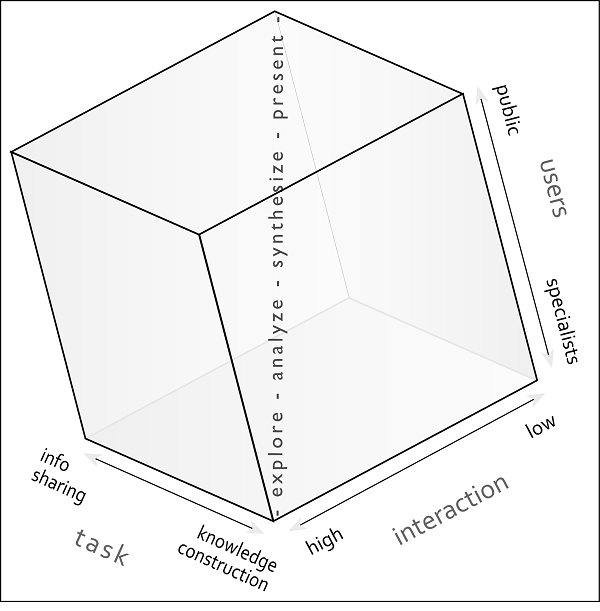
\includegraphics[width=\linewidth]{img/CV35-Fig2a-600.png}
\caption{\og \textit{An update to Cartography³, 10 years after its conception}\fg{}, par \cite{coltekin_geovisualization_2018}, d'après \cite[10]{maceachren_geovisualization_2004}.}
\label{fig:cartography3}
\end{minipage} \hfill
\begin{minipage}[t]{.46\linewidth}
\centering
\captionsetup{width=.9\linewidth}
\vspace{0pt}
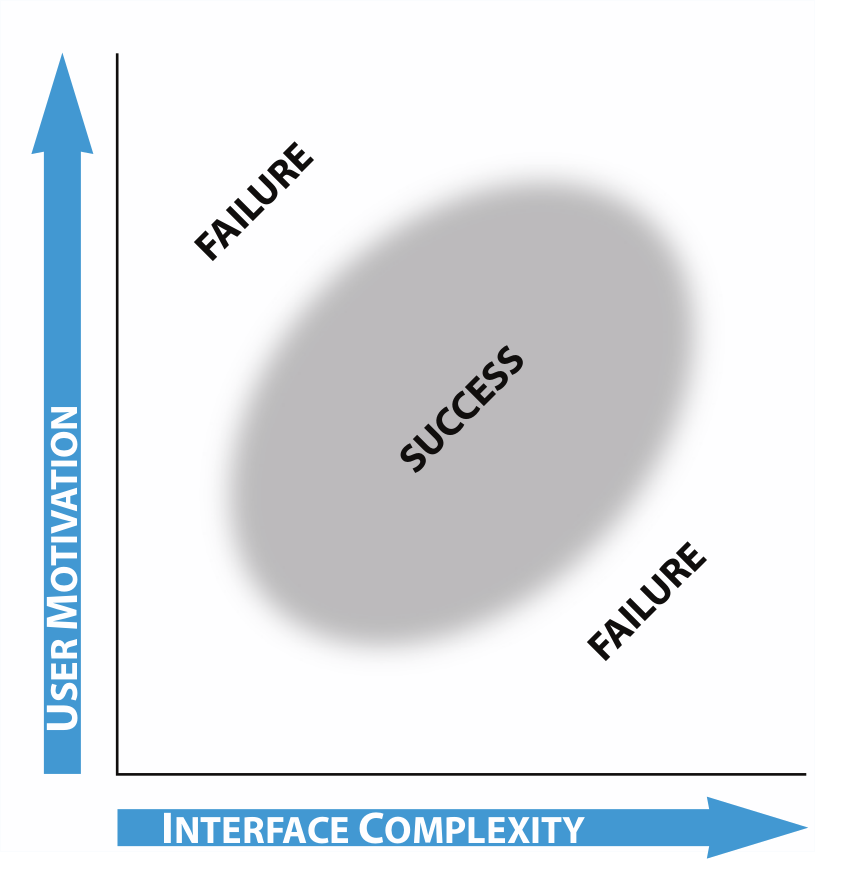
\includegraphics[width=\linewidth]{img/Roth_Interface_Complexity.png}
\caption{\og \textit{Interface complexity versus user motivation. }\fg{}, \cite[79]{roth_interactive_2013}.}
\label{fig:interface-complexity}
\end{minipage}
\end{figure}

L'usage prévu de SimEDB -- nettement dans la construction de connaissance --, de même que le \og niveau\fg{} de ses utilisateurs -- expert dans le sens thématique et de la modélisation conceptuelle --, devraient donc logiquement, selon le schéma, bénéficier d'une forte complexité possible dans l'interaction.

\paragraph*{Des utilisateurs hétérogènes mais captifs}

SimEDB s'inscrit pourtant à un niveau intermédiaire, entre l'analyse et la synthèse : l'exploration, au sens entendu par MacEachren (\textit{explore}), est ici délaissée de par le choix de présenter des indicateurs spécifiés plutôt que de laisser l'utilisateur les assembler.

Cet écart au modèle conceptuel de MacEachren s'explique notamment par la diversité des utilisateurs de SimEDB : qualifier un niveau d'expertise général serait absurde, tant les spécificités de cette expertise sont nombreuses : entre des profils de spécialiste thématiciens, de modélisateurs ou encore de géomaticiens, l'expertise est présente, mais concernant des champs différents, toutefois tous intéressés par l'exploration des sorties de SimFeodal.

Il est dès lors peu évident de se fixer sur un degré de complexité à atteindre dans la plate-forme d'exploration : un niveau faible serait frustrant pour les utilisateurs avancés, et un niveau avancé serait source de confusion et donc de perte de motivation.

Il nous était toutefois possible de miser sur une bonne motivation générale étant donné les circonstances particulières d'utilisation de SimEDB : contrairement à une utilisation grand public, qui ne présente aucun engagement vis-à-vis d'une interface d'exploration de données, ou à l'inverse contrairement à des domaines experts où chaque utilisateur dispose de ses propres outils et méthodes pour explorer un jeu de données, le public cible de SimEDB est \og captif\fg{}, c'est-à-dire qu'il ne dispose pas d'autre solution que de passer par cette plate-forme pour explorer les données, en particulier en raison des contraintes liées à ces données (cf. \cref{subsec:donnees-indicateurs}, \cnameref{subsec:donnees-indicateurs} par exemple).

Dès lors, la motivation des utilisateurs ne peut qu'être importante, et l'interface a la possibilité de devenir plus complexe tout en se révélant adaptée (\cref{fig:interface-complexity}).

\paragraph*{Intuititivé de l'usage au regard des applications traditionnelles}

En dépit de cette motivation, les utilisateurs de SimEDB demeurent majoritairement des experts thématiciens, potentiellement peu familiarisés à l'exploration de données interactives.
Afin que le temps d'exploration des données issues de SimFeodal soit dévoué à la compréhension et à la synthèse de ces données plutôt qu'à un apprentissage ou amélioration en exploration de données, il a été choisi de créer une application aussi simple que possible au regard des fonctionnalités principales qu'elle devait permettre : observer les indicateurs de sortie de simulation pour des expériences données, et les comparer entre elles aussi efficacement que possible.
Il n'était donc pas question de construire un nouveau \og logiciel expert \fg{}, doté de dizaines de fonctionnalités avancées, mais au contraire, de simplifier au maximum l'interface pour ne pas encombrer et complexifier l'utilisation de ces fonctionnalités principales.
On souhaitait une plate-forme aussi épurée que possible, plutôt que de partir, par exemple, sur la personnalisation et adaptation de l'un des outils d'exploration existants et dédiés à offrir une forte possibilité de manipulation.

\subsubsection{Efficacité}

Dans la description du choix du SGBD, on a mentionné une première fois l'intérêt de disposer d'une solution d'interrogation de données permettant une rapidité de l'exécution des requêtes.
Sans entrer dans le détail des recherches en IHM, on peut toutefois caractériser cet intérêt par deux aspects complémentaires, une solution interactive minimisant les latences permettant (1) de conserver l'utilisateur, c'est-à-dire de ne pas le décourager d'utiliser l'application, et (2) de lui faire conserver sa concentration (\textit{focus}), c'est-à-dire que le délai entre son interaction et la réponse graphique soit suffisamment court pour que l'identification effectuée par son système cognitif ne soit pas affecté.

Le premier point a été abordé plus haut (\cref{subsubsec:interroger-robuste-efficace}), et surtout, en raison de la \og captivité\fg{} de l'utilisateur évoquée ci-dessus, ne s'applique que marginalement à notre cas d'étude : si des délais trop importants pourraient décourager l'utilisateur, l'absence d'alternative utilisable pour explorer ces données les contraint toutefois à faire usage de la plate-forme d'exploration pour comprendre le comportement du modèle SimFeodal.

\paragraph*{Conserver la concentration}

Le problème de la concentration de l'utilisateur demeure, lui, critique : des études ont montré, depuis longtemps \autocite{mackenzie_lag_1993}, qu'il y avait un lien fort entre la performance d'une interrogation visuelle et le délai nécessaire à son obtention.
\cite[8]{liu_effects_2014} montrent ainsi qu'avec un simple délai de $500ms$, la qualité des observations, des généralisations qui peuvent être tirées des données, et des des hypothèses émises, décroît nettement. Les auteurs indiquent d'ailleurs que ces effets sont plus importants encore quand l'exploration est effectuée par des actions de \textit{brushing} et de sélections croisées (\textit{linking}), deux méthodes qui sont au cœur de SimEDB : \og For example, more aggressive caching or prefetching methods may be employed for operations sensitive to small variations in latency, such as brushing and linking \fg{}\autocite[9]{liu_effects_2014}.

\cite{forch_are_2017}, pour leur part, étudient la perception du délai de réponse lors d'interactions menées avec une souris d'ordinateur. Ils concluent ainsi que les utilisateurs perçoivent des délais d'attente inférieurs à $100ms$, mais notent que les utilisateurs n'en sont pas pour autant perturbés, en particulier ceux qui ont le moins l'habitude de réactions rapides\footnote{
Ils remarquent ainsi que les utilisateurs plus habitués à des jeux vidéos rapides (\og highly dynamic computer games, such as action games, racing games, or first person shooter games [...]\fg{}, \cite[51]{forch_are_2017}) sont plus vite affectés par le délai de réponse que les autres.
}.

Concernant le champ, plus spécifique, des \textit{visual analytics}, nous n'avons pas trouvé d'articles de référence permettant d'établir une comparaison de l'efficacité des résultats trouvés selon la latence de la réponse.
Les auteurs de ce champ recommandent de prêter attention à la rapidité de rendu et à son optimisation, mais sans que ne trouvions de résultats plus précis :
\begin{quotation}
\og
When simple pattern finding is needed, the importance of having a fast, highly interactive interface cannot be emphasized	enough. If a navigation technique is slow, then the cognitive costs can be much greater than just the amount of time lost, because an entire train of thought can become disrupted by the loss of the contents of both visual and nonvisual working memories.
\fg{}\\
\mbox{}~ \hfill  \cite{ware_information_2012}, tiré de \cite[12]{amirpour_amraii_human-data_2018}.
\end{quotation}

Tout au plus pouvons-nous émettre l'idée qu'il serait évident que la latence acceptée dans un environnement graphique de ce type soit largement supérieure à celle des environnements virtuels (réalité augmentée, visualisations immersives\ldots), sans pour autant que nous ne puissions quantifier cet écart.
\cite[74]{shneiderman_designing_2004} indiquent tout de même, parmi les \og 8 règles d'or du design d'interfaces\fg{} un délai maximal pour une phase d'exploration, sur lequel nous pouvons construire une estimation : \og \textit{Reduce short-term memory load.} The limitation of human information processing in short-term memory (\textbf{the rule of thumb is that humans can remember ``seven plus or minus two chunks'' of information}) requires that displays be kept simple, multiple-page displays be consolidated, window-motion frequency be reduced, and sufficient training time be allotted for codes, mnemonics, and sequences of actions.\fg{}.
Si l'on considère qu'une session d'exploration requiert l'étude d'une dizaine d'indicateurs, et que chacun demande une quinzaine de secondes d'analyse visuelle, alors le temps d'attente entre les visualisations ne doit pas dépasser deux à trois secondes.

Selon ces différentes considérations, dans le cadre de SimEDB, on doit donc viser à développer une plate-forme aussi rapide que possible, tout en sachant, dès le départ, qu'il sera impossible d'arriver aux délais de $100ms$ ou $500ms$ évoqués précédemment, ne serait-ce que parce que le temps de requête des données -- sans compter le temps de rendu graphique -- est déjà supérieur d'un ordre de grandeur.

\subsubsection{Interopérabilité et évolutivité}

Une autre contrainte forte tient cette fois au choix de l'environnement informatique qui accueillera la plate-forme d'exploration.
On peut résumer ce choix à deux alternatives : un environnement local, en installant l'application sur l'ordinateur de chaque utilisateur, ou un environnement distant, où l'application serait donc accessible à distance, par exemple via une interface web.

Ce choix a des nombreuses répercussions, aussi bien en matière de possibilité d'accès que de facilité à faire évoluer la plate-forme.
Le choix le plus classique est de développer une application installable sur un ordinateur : cela permet de garantir une utilisation à tout moment, sans contrainte d'accès au réseau internet, et cela permet aussi d'obtenir de meilleurs performances, puisque la rapidité de l'application dépendrait uniquement de la puissance de l'ordinateur plutôt que de devoir souffrir du passage par l'intermédiaire d'un serveur.

\paragraph*{Différents supports d'interrogation}
La performance d'une application locale, par rapport à une application distante, est un atout extrêmement intéressant, comme on vient de le montrer plus haut.
Pourtant, cela implique une énorme contrainte : l'application doit être interopérable entre les différents systèmes d'exploitations (\textit{Operating System}, OS) et versions de ceux-ci.
Les utilisateurs potentiels de SimEDB, représentation fidèle des acteurs de la recherche, se partagent ainsi entre les trois systèmes d'exploitations majoritaires (Windows, MacOs, Linux).

Pour permettre à chacun d'utiliser SimEDB, il faudrait donc que le développement de cette plate-forme soit compatible avec ces différents OS, ce qui est une contrainte considérable en développement logiciel.

Ne mentionnons même pas les nouveaux OS, centrés autour d'usages tactiles, tels qu'on les retrouve sur les tablettes et autres \textit{smartphones}, qui demandent, eux aussi, de nombreuses spécificités de développement.

En somme, disposer d'une application locale universelle, c'est-à-dire utilisable quelque soit le support informatique, est une quasi-impossibilité technique, et un objectif en soit, que notre travail de recherche ne cherche aucunement à résoudre.
Pour garantir la faisabilité d'une plate-forme d'exploration de données locale dédiée aux données de simulation de SimFeodal, il faudrait donc commencer par restreindre son champ d'application à un ou deux supports officiels, par exemple l'OS Windows, abandonnant de fait les utilisateurs potentiels ne disposant pas de cette architecture logicielle.

\paragraph*{Gérer les mises à jours et modifications}

Comme pour les bases de données (\cnameref{par:stockage-centralise}, \cpageref{par:stockage-centralise}), la question de l'application locale ou distante pose un contrainte supplémentaire en matière de maintenabilité et d'évolutivité de la plate-forme choisie : dans le cadre d'une application locale (correspondant au distribué en SGBD), la distribution des différentes mises à jour de l'application entraînent nécessairement l'installation locale, à chaque fois.
Le risque est alors que tous les utilisateurs ne disposent pas d'une même version, ce qui peut entraîner, par exemple, des contradictions dans l'évaluation d'expériences, certains utilisateurs ayant accès à une version \og buggée\fg{}.

Sans aller jusqu'à ces extrêmes, notons qu'avec une application locale, le temps de répercussion d'une modification du code de la plate-forme est plus important : il faut en effet réinstaller sur chaque poste le logiciel ainsi modifié.
Cela disqualifie de fait des modifications \og en direct\fg{}, par exemple lors d'une session collective d'exploration des résultats où les utilisateurs auraient des propositions de modifications à faire, ne serait-ce que pour des changements aussi infimes que des titres de graphiques ou d'axes.

\paragraph*{Le choix d'une application web}

Au contraire, avec une application distante, donc basée sur l'accès, par un navigateur internet, à une application centralisée, ces problèmes ne se posent pas : des navigateurs sont disponibles pour tous les OS existants (OS dédiés aux ordinateurs ou aux usages mobiles), et interprètent de la même manière une page web, indépendamment de leur support de consultation.
De plus, comme pour les SGBD, l'usage d'une plate-forme distante permet une répercussion instantanée des mises à jour et corrections : un utilisateur n'a qu'à rafraichir sa page pour que la dernière version de l'application s'affiche.
De la même manière, si un utilisateur souhaite étudier un nouvel indicateur, non prévu auparavant, le temps de déploiement peut être suffisamment court pour que cela soit possible au cours d'une même session d'exploration de données.

Il y a toutefois un désavantage certain, puisque les données permettant l'affichage des indicateurs doivent transiter sur le réseau internet : l'application n'est donc pas disponible hors-connexion, et, en cas de connexion lente, sera particulièrement éprouvée.
Cette lenteur relative est toutefois compensée par un avantage à la centralisation de l'application : les calculs, parfois lourds, ne reposent pas sur les capacités individuelles des ordinateurs clients.
En installant l'application sur un serveur dédié, il suffit donc d'augmenter les caractéristiques de celui-ci pour que les performances soient améliorées pour chacun des utilisateurs de l'application.

Dans le cas de SimEDB, nous disposons de ressources informatiques largement suffisantes (serveur de calcul interne à l'UMR Géographie-cités dans un premier temps, puis serveur de calcul partagé via la \og Très Grande Infrastructure de Recherche\fg{} -- TGIR -- Huma-Num) pour assurer une rapidité de traitement des données et ainsi permettre à l'application SimEDB de se dégager de ce \og goulot d'étranglement\fg{} technique qu'aurait sinon éprouvée la plate-forme.

\subsubsection{Généricité de l'interrogation et indépendance aux données}

La dernière contrainte, plus technique, tient au besoin de généricité d'une plate-forme d'exploration de données vis-à-vis des données qu'elle interroge.
On a résumé les possibilités et choix effectués en matière de SGBD (\cref{subsec:capacite-interrogation} :  \cnameref{subsec:capacite-interrogation}), et décidé de ne retenir que des SGBD permettant une interrogation standardisée via des connecteurs génériques et un langage universel (le SQL).

L'infrastructure de stockage et d'organisation des données a ainsi été conçue pour être aussi générique que possible.
Encore faut-il que la plate-forme d'exploration de données soit elle aussi aussi générique que possible, et donc en mesure de profiter de l'universalité du SGBD choisi.

\paragraph*{Indépendance au support de données}
Une contrainte forte est donc constituée par la capacité de la plate-forme a être indépendante de la source des données : quelque soit le SGBD choisi, les requêtes émises par la plate-forme doivent être les mêmes, sans requérir d'adaptations spécifiques en dehors de la désignation du lieu de stockage des données	et des pilotes du SGBD.

Dans les faits, lors de la construction de SimEDB (cf. \cref{sec:explorer-sorties-simfeodal} : \cnameref{sec:explorer-sorties-simfeodal}), plusieurs solutions de stockage de données ont été utilisés successivement : de simples fichiers csv au départ jusqu'au SGBD ultra-performant MapD, en passant par des solutions plus classiques intermédiaires (SQLite et MonetDB notamment).

Il n'était donc aucunement question d'avoir à modifier le code source permettant de générer les indicateurs depuis les données, mais au contraire, de s'assurer d'utiliser des bibliothèques logicielles indépendantes des données, c'est-à-dire capables d'exécuter les mêmes chaînes de traitements quelque-soit la provenance des données.

\paragraph*{Indépendance aux requêtes et modularité de l'implémentation}\label{par:DSL}

Pour garantir cette généricité, il est donc nécessaire de s'assurer que le mode de communication de la plate-forme vers les données soit bien basé sur un langage universel : le SQL.
Il convient donc de choisir un ensemble de technologies permettant de générer des requêtes SQL, quand bien même l'expression de ces requêtes elles-mêmes serait conçue dans un autre langage.
Faire appel à un langage intermédiaire, générant du SQL en sortie depuis une entrée sous forme d'un \og \textit{Domain Specific Language}\fg{} (DSL) permet ainsi de bénéficier d'une part de l'universalité du SQL, et d'autre part, d'une syntaxe plus expressive que celle du SQL.
Pour les requêtes complexes, le SQL tend ainsi a être peu lisible, les opérations s'emboîtant les unes dans les autres de manière très linéaires, et donc, souvent verbeuses.
En SQL pur, il est donc peu évident de créer une implémentation modulaire d'une requête, c'est-à-dire permettant une factorisation des commandes et un paramétrage des entrées.

Les indicateurs de sortie de SimFeodal sont pourtant, on l'a vu, assez fréquemment basés sur le même type d'opération : variation du nombre moyen d'agents au cours du temps de la simulation, courbes rang-taille des hiérarchies d'un type d'agent etc.
Dans le cas du premier exemple, en SQL, pour passer d'une requête permettant de récupérer le nombre de foyers paysans au cours du temps, groupés par année et avec un filtre sur certaines simulations, il ne faut que quelques lignes de code. Pour adapter cette requête à l'interrogation du nombre d'agrégats, dans les mêmes conditions d'agrégation et de filtrage, l'effort est minime, mais peu évident à paramétrer pour rendre cette démarche plus générique.

En utilisant un DSL, plus adapté à la manipulation de données qu'à la sélection de sous-ensembles, on gagne donc en modularité d'implémentation , et donc en ré-utilisation de fonctions plus génériques, ce qui permet de disposer d'un code-source plus robuste, ré-utilisable et évolutif.

\subsubsection*{Conclusion : Vers une plate-forme web générique et intuitive}

Il ressort de ces différentes contraintes et choix d'utilisation que les choix techniques, propres aux modalités d'interrogation des bases de données, mais aussi méthodologiques, au regard de la conception d'une interface graphique intuitive, imposent des restrictions assez conséquentes sur les possibilités techniques disponibles pour la conception de la plate-forme SimEDB.
En premier lieu, on fait le choix de se tourner vers une plate-forme implémentée sous forme d'application web, utilisable depuis un simple navigateur -- donc inter-opérable entre les différents supports technologiques --, ce qui exclue de fait quantités d'outils, de logiciels et de bibliothèques logicielles pensées pour l'exploration interactive de données.
On souhaite de plus que la plate-forme utilisée dispose d'une interface aussi épurée que possible, donc nécessairement très adaptée au cas particulier des données issues de SimFeodal, ce qui là aussi élimine un ensemble de solutions \og clefs-en-main\fg{}, par exemple conçues autour des \og webSIG\fg{} ou de bibliothèques logicielles de visualisations interactives intégrées.
L'utilisation de la plate-forme doit être aussi efficace que possible, en cherchant à minimiser les temps de latence entre sélection interactive et affichage des indicateurs en résultant.
On devra donc privilégier des ensembles technologiques récents et performants, intrinsèquement dédiés à l'interactivité, au détriment de \textit{frameworks} plus génériques, conçus pour une forte diversité d'usage plutôt que pour la tâche très spécifique que constitue la manipulation interactive de données.
Enfin, il faut que cette solution, dans la mesure du possible, soit en mesure de proposer une syntaxes d'interrogation de données modulaire, factorisée, et plus expressive que le SQL qu'elle doit pourtant réussir à générer.


\subsection{Construire une plate-forme interactive pour l'évaluation de SimFeodal}

Dans cette dernière sous-partie, nous allons donc présenter les choix -- techniques, esthétiques et interactifs -- qui ont été adoptés dans la conception et l'implémentation de SimEDB.
Nous les présentons ici de manière linéaire, dans l'ordre quasi-chronologique du développement, mais il est important de garder en considération que ces éléments sont intimement intriqués : un choix technique conditionne les types d'interactions possibles, l'utilisation de telle méthode d'interaction peut restreindre l'étendue des possibles techniques etc.

Notons enfin que l'application SimEDB présentée ici, aussi bien dans son usage que dans sa conception, représente un instantané de développement, qui correspond à la période de rédaction du présent chapitre :
à l'instar d'un modèle, une plate-forme peut et doit évoluer pour s'adapter aux besoins de ses utilisateurs tant qu'elle est utilisée.
Les technologies et choix esthétiques introduits n'ont pas toujours été présents, et auront sans doute à évoluer dans la suite de la \og durée de vie\fg{} de SimEDB.

\subsubsection{Choix des technologies}

Nous présentons ici les technologies mobilisées dans le cadre du développement de SimEDB.
Le but n'est pas d'entrer dans les détails de l'implémentation\footnote{
Le code source de SimEDB -- et l'historique de son versionnement -- sont, pour cela, disponible en ligne sous licence libre, sur la plate-forme Github : 
\faGithub~\href{https://github.com/RCura/SimEDB}{github.com/RCura/SimEDB}
}, mais bien de justifier et présenter les choix relatifs aux technologies employées, en restant donc à un niveau assez général\footnote{
À ce titre, les quelques lignes de codes présentes par la suite servent un but illustratif et descriptif, et nous semblent remplir ce rôle bien plus efficacement que n'importe quel schéma structurel ne le pourrait.
}.
Il nous paraît important d'entrer dans ces choix qui relèvent plus de la technique que de la méthodologie en ce qu'ils concourent de la volonté de reproductibilité de la thèse, et particulièrement de la reproductibilité de la démarche, conceptuelle et méthodologique, mise en place.
Nous portons la conviction que l'ensemble de technologies assemblées ici dans notre \og chaîne de traitement\fg{} est très largement ré-utilisable, dans le cadre d'adaptations à d'autres cas d'études, mais aussi et surtout, pour une multitude de problématiques requérant une évaluation visuelle de données massives (\hl{on y reviendra dans le chap 7}).

\paragraph*{Technologies webs \og natives\fg{}  et adaptativité}

Au cours de la dernière décennie, les interfaces physiques de consultation de médias informatiques se sont largement diversifiées.
Cela a provoqué une hétérogénéisation importante aussi bien des modes d'interaction (dispositifs \og tactiles\fg{}) que des modes d'affichages (les tailles et résolutions des écrans n'ont jamais été aussi diverses et imprévisibles).
En conséquence, les normes de présentations graphiques ont évolué, vers plus d'\fg{}adaptativité\fg{}, en particulier avec l'avènement du \og responsive web design\fg{} (\og conception de sites web adaptatifs\fg{}) qui permet de prévoir efficacement l'agencement d'une page web quelque soit le support de consultation.

Ces technologies, aujourd'hui indispensables, reposent sur des codes standardisés, verbeux et peu explicites, qui peuvent être générés à la volée par des \textit{frameworks} graphiques qui en simplifient l'usage.

Les technologies plus lourdes qui prédominaient dans la réalisation d'applications web interactives il y a quelques années (\texttt{Adobe Flash}, \textit{applets} Java\ldots) sont donc maintenant assez peu universelles et le niveau de développement de standards tels que le langage et environnement HTML5 a suffisamment augmenté pour pouvoir justifier de s'en passer.

Nous avons donc fait le choix de nous concentrer sur des environnements standardisés, capables de générer du \texttt{HTML} (\og \textit{HyperText Markup Language}\fg{}), lui-même mise en forme à l'aide de styles \texttt{CSS} (\og \textit{Cascading Style Sheets}\fg{}) et rendu interactif par du code \texttt{JavaScript}.

À ce titre, le framework \texttt{Bootstrap}\footnote{\href{http://getbootstrap.com/}{http://getbootstrap.com/}} s'est révélé extrêmement utile dans le \textit{design} de l'interface de SimEDB (et des versions précédentes), tant il simplifie l'expressivité d'une mise en page à l'aide d'une grille graphique et de composants interactifs ré-utilisables.

\paragraph*{Le choix d'environnements de développement intermédiaires}

\hl{Ne pas oublier, dans le positionnement (chap1) de consacrer au moins un paragraphe (ou encadré) au choix \og militant\fg{} de ne se tourner QUE vers des outils libres, sans exception.}

Pour construire des applications interactives en lignes, de multiples choix sont possibles, et l'on peut les catégoriser selon le niveau de développement qu'ils demandent.

Par exemple, il est tout à fait possible de s'appuyer sur des briques logicielles de bas niveau (ce que l'on appelle communément \textit{framework}), et de développer à partir de celles-ci toute l'interface et le fonctionnement d'une application, par exemple au sein de \textit{frameworks} \og MVC\fg{} (Modèle-Vue-Contrôleur).
Cette approche, majoritaire dans la construction d'applications actuelles (avec des \textit{frameworks} JavaScript tels que \texttt{ReactJS} ou \texttt{AngularJS}, ou encore Python tels \texttt{Django} ou \texttt{Flask}), est extrêmement flexible et performante, au prix d'un développement important : le \textit{framework} fournit des \og briques\fg{} logicielles de base -- les composants --, très génériques, qui doivent être largement adaptées.
La communication entre ces composants doit être entièrement prévue et implémentée, et on abouti donc nécessairement sur des projets assez importants, qui demandent une réelle expertise en développement et portent le risque d'être trop complexes pour être facilement adaptés et donc génériques.

À l'autre bout du gradient de développement, on peut aussi choisir de bâtir une application à partir d'un ensemble logiciel intégré, comme \texttt{Tableau}, qui permet d'agencer visuellement et graphiquement des composants graphiques et leurs liens. Ces outils, très usités en informatique décisionnelle, sont extrêmement simples à prendre en main, y compris pour des \og utilisateurs finaux\fg{} -- analystes par exemple --, mais sont en contre-partie bien moins personnalisables, adaptables, et sont majoritairement des logiciels propriétaires, donc non adaptables.

Entre ces deux extrêmes, quelques \textit{frameworks} intermédiaires, souvent originaires des outils de manipulation de données plus que du monde de l'informatique décisionnelle, mettent à disposition de l'utilisateur des composants de plus haut-niveau que les \og briques élémentaires\fg{}, où l'interaction entre les composants est déjà pré-conçue, tout en reposant sur une construction \og depuis zéro\fg{}, donc personnalisables et adaptables.
Généralement, chaque \textit{framework} est associé à un langage de programmation : \texttt{Shiny}\footnote{\href{https://shiny.rstudio.com/}{https://shiny.rstudio.com/} -- \cite{chang_shiny_2015}} pour le langage \texttt{R}, \texttt{Dash}\footnote{\href{https://plot.ly/products/dash/}{https://plot.ly/products/dash/} -- \cite{plotly_introducing_2017}} pour le langage \texttt{Python} et \texttt{Escher}\footnote{\href{http://escher-jl.org/}{http://escher-jl.org/}-- \cite{gowda_escher_2018}, d'après \cite{bezanson_julia_2014}} pour le langage \texttt{Julia}.

Le choix de tel ou tel framework dépend certes de la maturité de chaque projet -- Shiny est à ce titre très en avance --, mais surtout du langage informatique que le concepteur de l'application souhaite utiliser.
Dans le cas de SimEDB, le créateur de la plate-forme est adepte du langage R (voir \cite{commenges_r_2014}) et pratique l'environnement Shiny depuis plusieurs années (voir \cite{cura_creer_2015}) : le choix d'utiliser ce framework était donc assez évident.	

\paragraph*{Manipuler les données avec \texttt{R} et \texttt{dplyr}}

Les langages de programmation, et en particulier les plus utilisés en analyse de données, reposent souvent sur une architecture logicielle modulaire : le langage constitue un cœur, autour duquel des bibliothèques logicielles (des \textit{packages} en R) viennent ajouter des fonctionnalités.
Parmi ces bibliothèques logicielles, en Python comme en R, certaines sont entièrement dédiées à la manipulation de données tabulaires, on parle alors de \og Data Manipulation Language\fg{} (DML) et permettent d'effectuer des traitements avec des approches fonctionnelles, plutôt qu'avec les structures impératives plus fréquemment utilisées en programmation.
En R, ces \textit{packages} constituent de véritables écosystèmes, dotés de leur propre DSL (voir \cnameref{par:DSL}, \cpageref{par:DSL}) et donc d'une grammaire de manipulation de données propre.

L'un de ces \textit{packages}, \texttt{dplyr} \autocite{wickham_dplyr_2015}, s'inscrit dans un écosystème dénommé \texttt{tidyverse} \autocite{wickham_tidyverse_2017}, et permet ainsi de chaîner des opérations de manipulation de données en une chaîne de traitement complète, plutôt que de faire appel aux habituelles boucles de parcours de matrices propres aux langages de programmation classiques.
Ce faisant, avec des opérations chaînées, qui reposent sur des \og verbes\fg{} permettant d'effectuer des traitements de restructurations, de modification, de filtrage ou d'enrichissement d'une donnée tabulaire, on obtient un ensemble d'instructions qui forment une \og phrase\fg{} de manipulation de données, exprimées donc dans la \og grammaire de traitement de données\fg{} fournie par \texttt{dplyr}.
Cette \og grammaire\fg{} s'inspire notamment du SQL, bien que beaucoup plus complète, et peut en particulier être \og convertie\fg{} en SQL (\cref{fig:dml-simedb}), c'est-à-dire qu'une suite d'instructions exprimées via dplyr en R (\cref{subfig:exemple-dplyr-R}) peut être traduite en SQL (\cref{subfig:exemple-dplyr-SQL}), et donc envoyée et exécutée sur un SGBD.

En matière de performance, l'approche de \texttt{dplyr} est intéressante : toutes les opérations sont effectuées par le SGBD directement, et seul le résultat final est renvoyé à R (instruction \texttt{collect()}).
Le traitement de données bénéficie donc de la rapidité d'exécution du SGBD MapD, tout en profitant de la syntaxe expressive de \texttt{dplyr}.

\begin{figure}[H]
\centering
\hspace{5pt}
\subfloat[Code source R avec le \textit{package} \texttt{dplyr}]{\label{subfig:exemple-dplyr-R}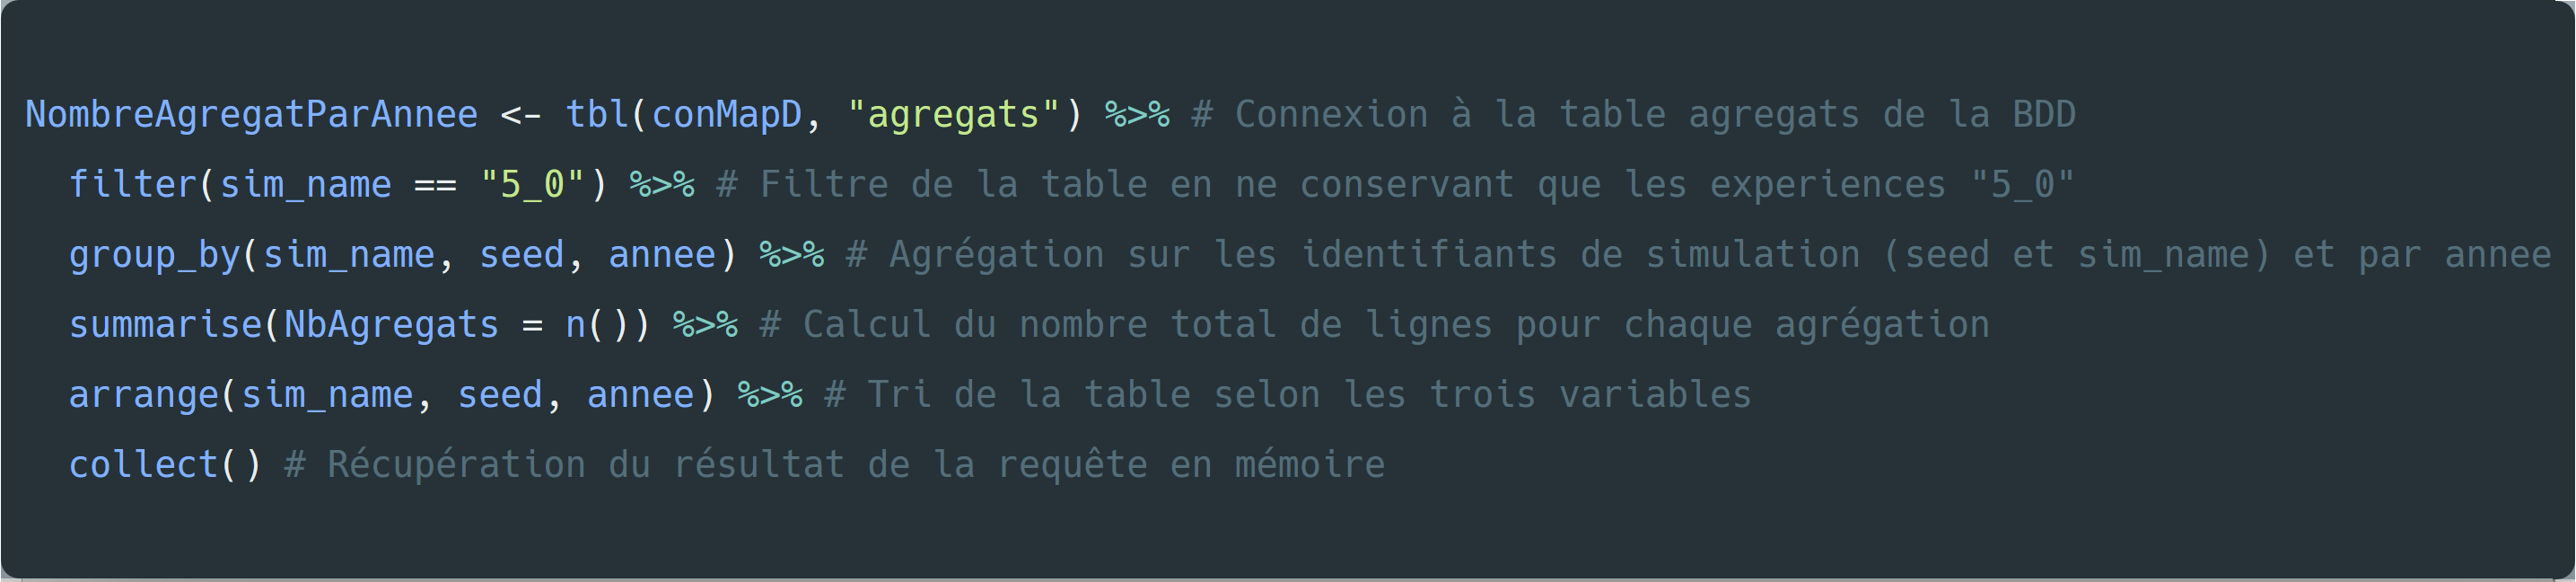
\includegraphics[width=\linewidth]{img/dplyr_cut.png}}
\hspace{5pt}
\subfloat[Traduction du code source \texttt{dplyr} en \texttt{SQL}]{\label{subfig:exemple-dplyr-SQL}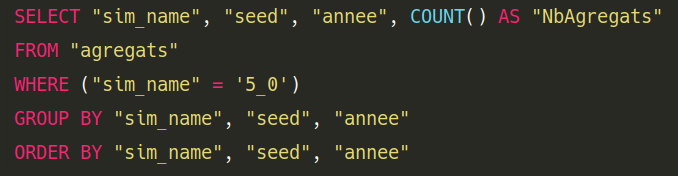
\includegraphics[scale=.35]{img/SQL_Sublime.png}}
\caption{Un exemple de manipulation de données stockées dans un SGBD depuis R. On y interroge la table des agrégats de population pour calculer le nombre moyen d'agrégats par année de simulation.}
\label{fig:dml-simedb}
\end{figure}

\clearpage
\paragraph*{Création de graphiques avec \texttt{ggplot2} et la \og \textit{grammar of graphics}\fg{}}

\paragraph*{}
\begin{wrapfigure}{l}{.42\linewidth}
\centering
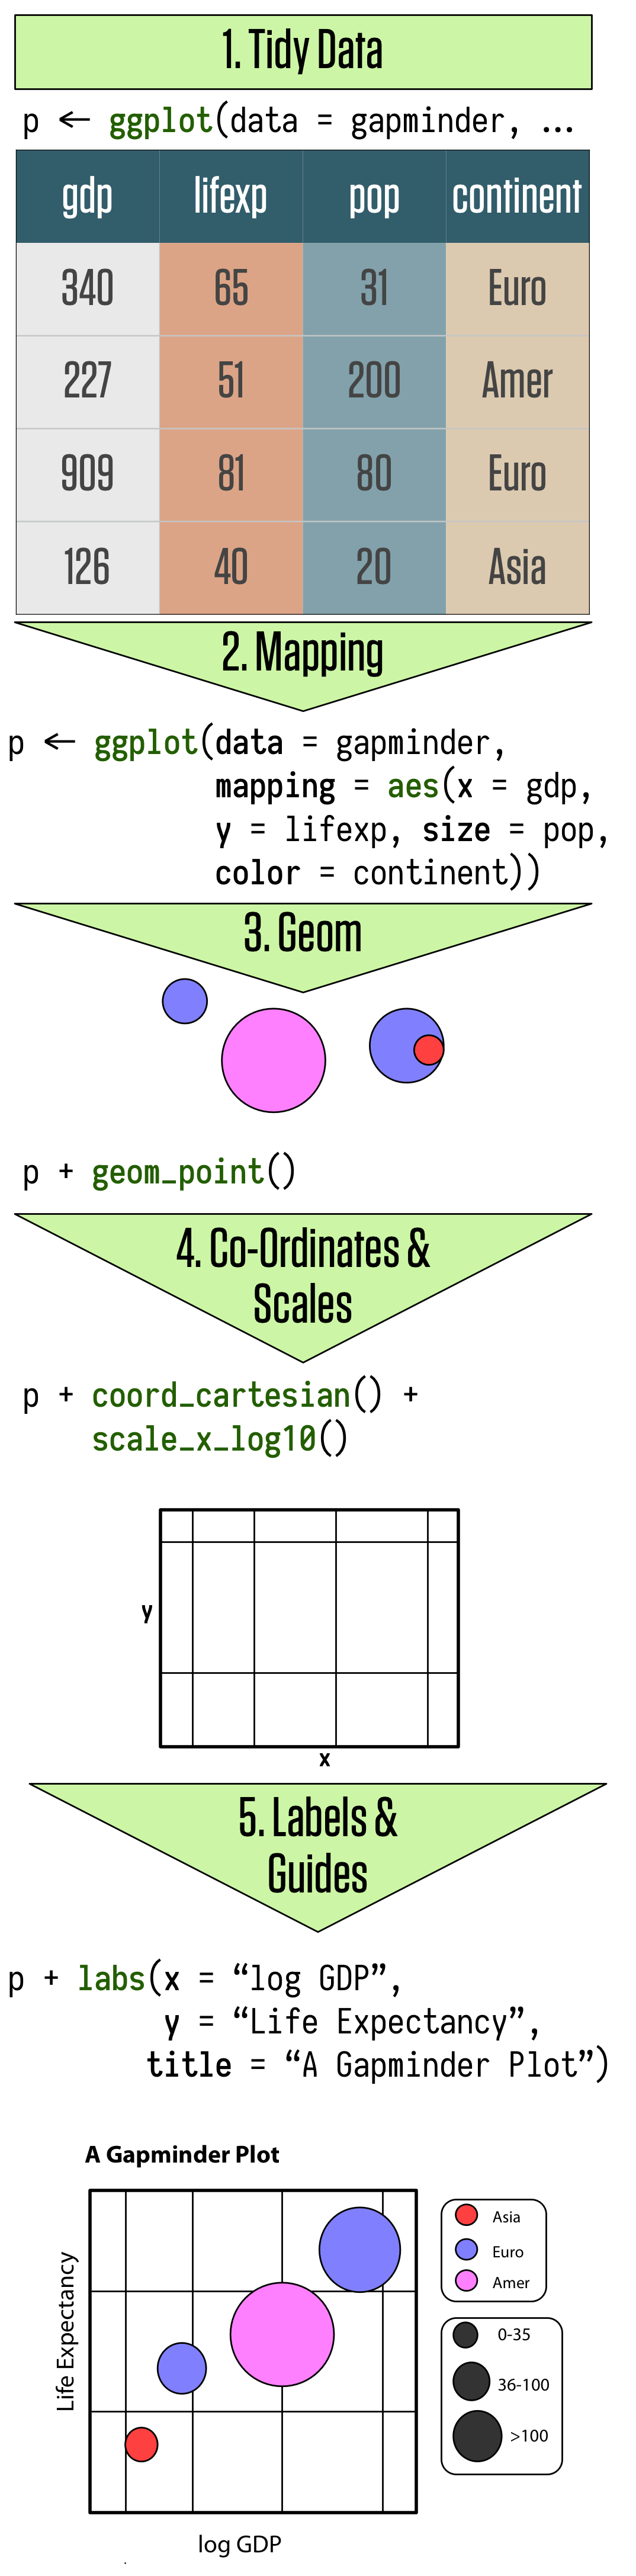
\includegraphics[width=.92\linewidth]{img/ch-03-ggplot-flow-vertical.png}
\caption{Représentation des éléments de grammaire de \texttt{ggplot2}, tiré de \cite{healy_data_2018}.\\
\hl{Ré-organiser proprement le graphique}%
}
\label{fig:socviz-ggplot2}
\end{wrapfigure}
Une fois les données pré-traitées, encore est-il nécessaire de construire les indicateurs graphiques de sortie de simulation.
Pour cela, il existe de nombreux \textit{packages} pour R dédiés à la représentation graphique.

L'un des \textit{packages} les plus utilisés, \texttt{ggplot2} \autocite{wickham_ggplot2_2016}, met en œuvre une syntaxe assez adaptée à nos contraintes : ce \textit{package} est conceptuellement fondé sur la \og \textit{grammar of graphics}\fg{}, c'est-à-dire une vision modulaire et très structurée de la conception graphique, pensée par Leland Wilkison \autocite{wilkinson_grammar_2006}.
La logique, assez familière pour un utilisateur de Systèmes d'Information Géographique (SIG), consiste à penser une représentation graphique comme un ensemble de couches (\textit{layers}), qui se superposent, se complètent, et sont toutes basées sur une source de données.
Les différentes composantes des données (variables par exemple) sont associées à des composantes graphiques de base (abscisse, ordonnée, taille, couleur \ldots), formant ainsi une \og cartographie\fg{} (\textit{mapping}) des données avec les composants graphiques (voir \cref{fig:socviz-ggplot2}).

Pour SimEDB, l'un des intérêts principaux de créer les indicateurs graphiques est justement cette grammaire, extrêmement structurée, qui permet donc de ré-utiliser largement les codes-sources écrits pour un indicateur et de les adapter aisément à d'autres indicateurs.
Par exemple, de nombreux indicateurs de sortie de SimFeodal montrent l'évolution du nombre d'agents au cours des années de simulation (\cref{fig:exemple-ggplot2-simedb}).
Ce type de graphique est rapide à produire avec \texttt{ggplot2} -- il ne requiert que quelques lignes de code (\cref{subfig:exemple-ggplot2-R}) --,
et en changeant le tableau de données en entrée (créé dans \cref{subfig:exemple-dplyr-R}), reproduit exactement le même type de graphique pour, par exemple, un autre type d'agent.
Le \textit{package} \texttt{ggplot2} répond tout à fait aux contraintes de modularité exposées plus haut, et permet de factoriser le code-source, ce qui garanti une maintenance plus rapide et une meilleure robustesse de l'application dans son ensemble.

\clearpage

\begin{figure}[H]
\centering
\hspace{5pt}
\subfloat[Code source R avec le \textit{package} \texttt{ggplot2}]{\label{subfig:exemple-ggplot2-R}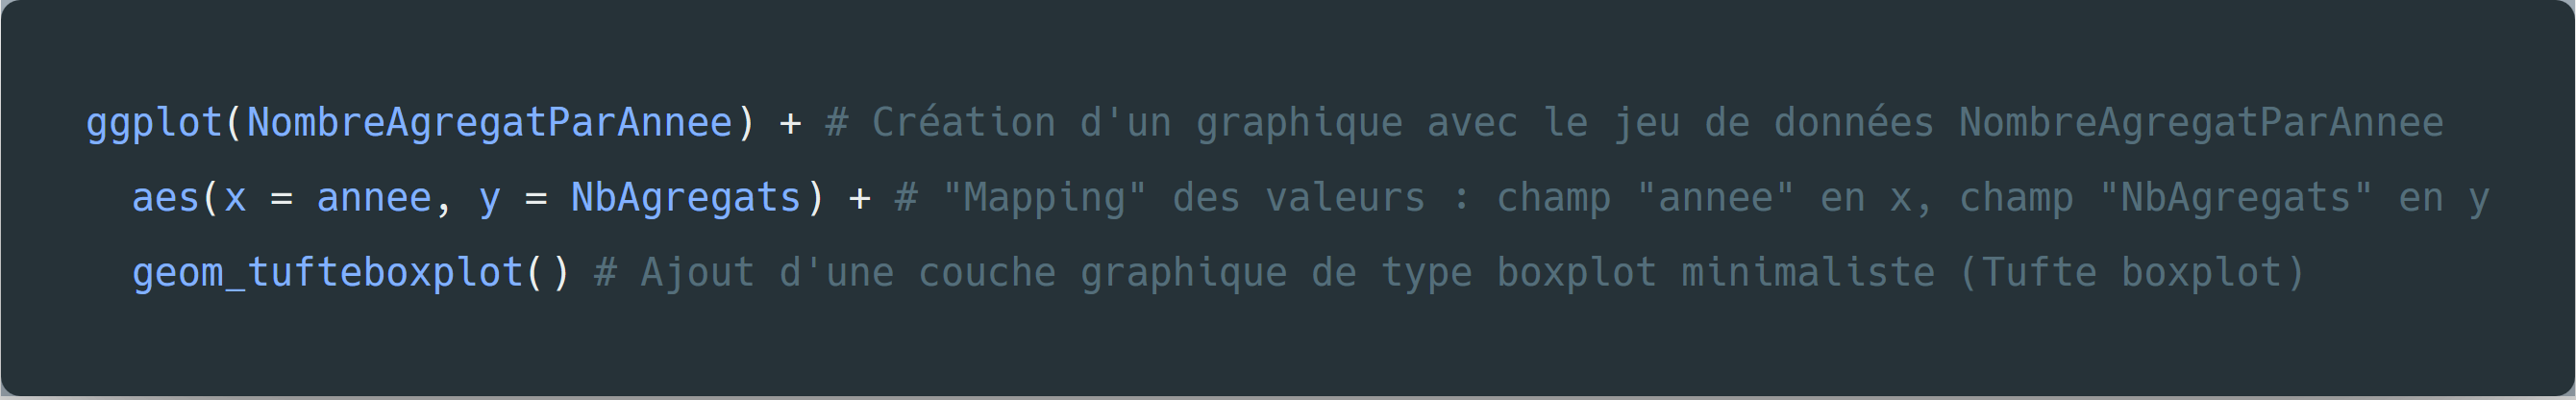
\includegraphics[scale=.15]{img/ggplot2.png}}
\hspace{5pt}
\subfloat[Graphique généré]{\label{subfig:exemple-ggplot2-plot}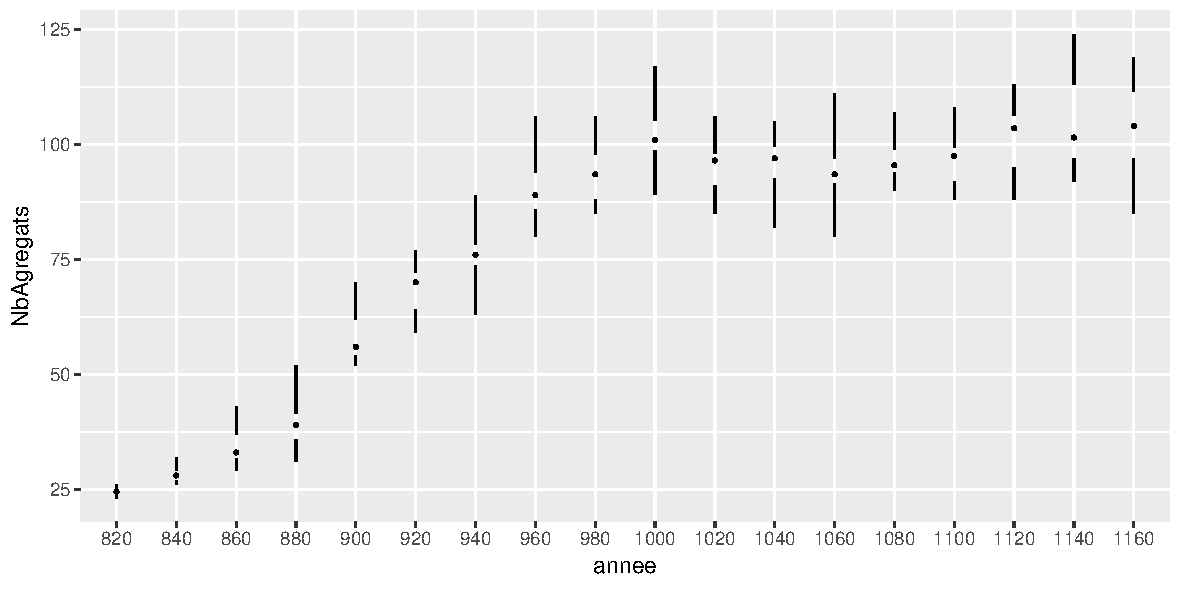
\includegraphics[width=\linewidth]{img/chap5_exemple_indicateur.pdf}}
\caption{Un exemple de manipulation de données stockées dans un SGBD depuis R.}
\label{fig:exemple-ggplot2-simedb}
\end{figure}

\paragraph*{Fluidifier les étapes de rendu : le \og pipeline de visualisation\fg{}}\label{par:visualisation-pipeline}


\Cite{dos_santos_gaining_2004} ont conceptualisé et schématisé l'ensemble des étapes nécessaires à la construction d'une visualisation, depuis les données brutes jusqu'à l'image finale, au sein d'un \og pipeline\fg{} de la visualisation (\cref{subfig:visualisation-pipeline}).

Dans la chaîne de traitement la plus classique, ces étapes s'effectuent au sein de différents logiciels, chacun dédiés à une tâche. Dans le domaine des utilisateurs de SIG, on retrouve par exemple fréquemment une préparation des données dans un tableur, un import dans un logiciel SIG qui va être chargé de la cartographie, puis un export vers un logiciel de dessin vectoriel afin de réaliser la mise en page.
À chaque changement de logiciel, il est nécessaire d'exporter les données produites, puis de les ré-importer dans le logiciel suivant.

A contrario, le propre de l'utilisation d'un langage de programmation plutôt que d'un outil graphique est de pouvoir automatiser et intégrer l'ensemble de ces étapes.
L'utilisation de \texttt{R} comme langage de développement de SimEDB nous permet ainsi de développer une unique chaîne de traitement, qui ne requiert aucun import/export de données, et peut donc être consolidée, vérifiée et surtout ré-employée \textit{ad libitum}.

L'enchaînement des \textit{packages} employées dans SimEDB est présenté dans la \cref{subfig:visualisation-pipeline-simedb}, et le code-source correspondant à l'exemple développé dans cette sous-partie dans la \cref{fig:visualisation-pipeline-exemple}.

\begin{figure}[H]
\centering
\hspace{5pt}
\subfloat[\og \textit{The Visualisation Pipeline}\fg{}, de \cite{keim_mastering_2010}, p.92, d'après \cite{dos_santos_gaining_2004}, p. 314 ]{\label{subfig:visualisation-pipeline}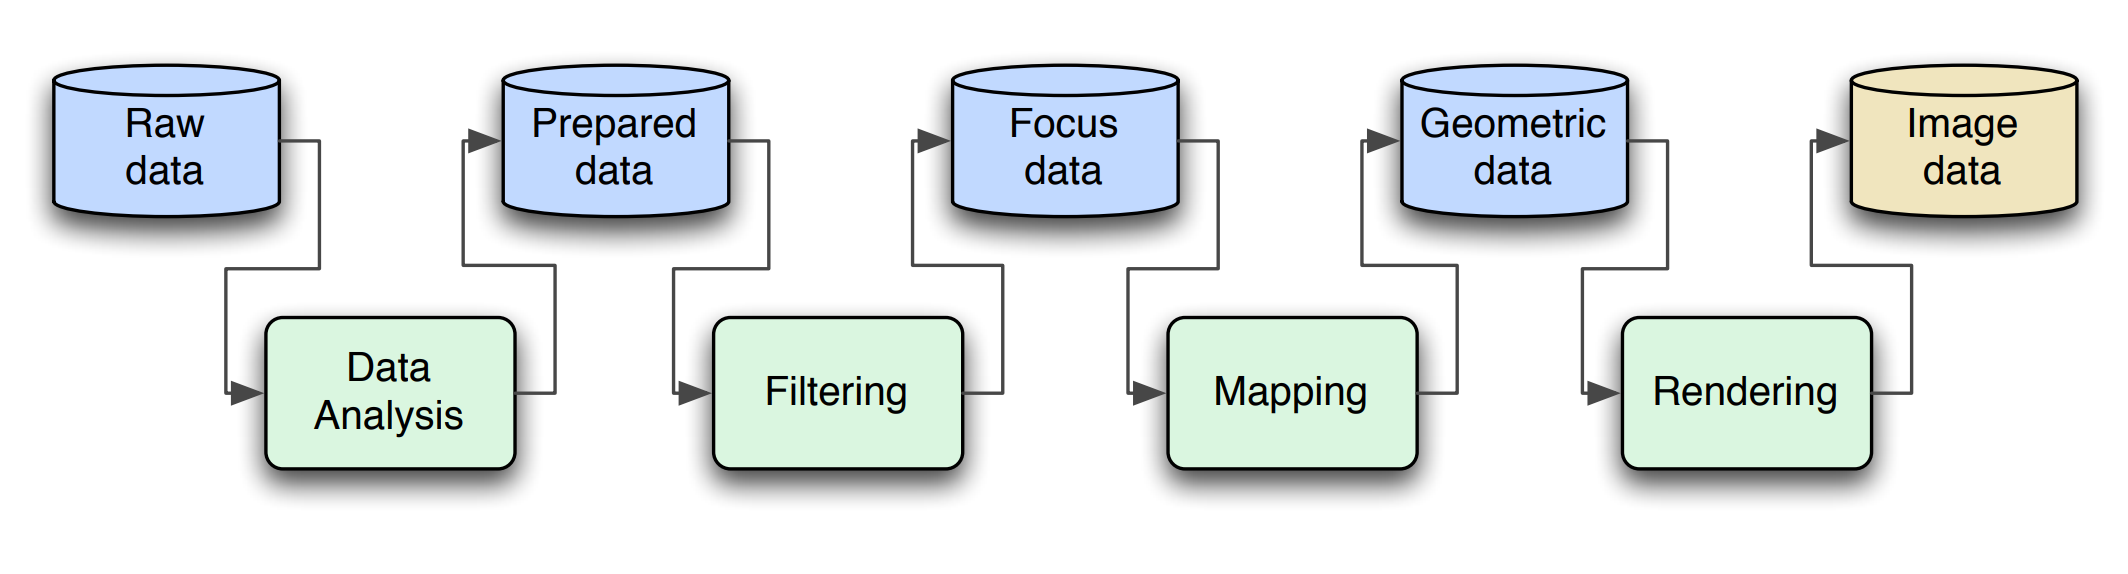
\includegraphics[width=\linewidth]{img/Visualisation_Pipeline_p92.png}}
\hspace{5pt}
\subfloat[Technologies utilisées dans SimEDB.]{\label{subfig:visualisation-pipeline-simedb}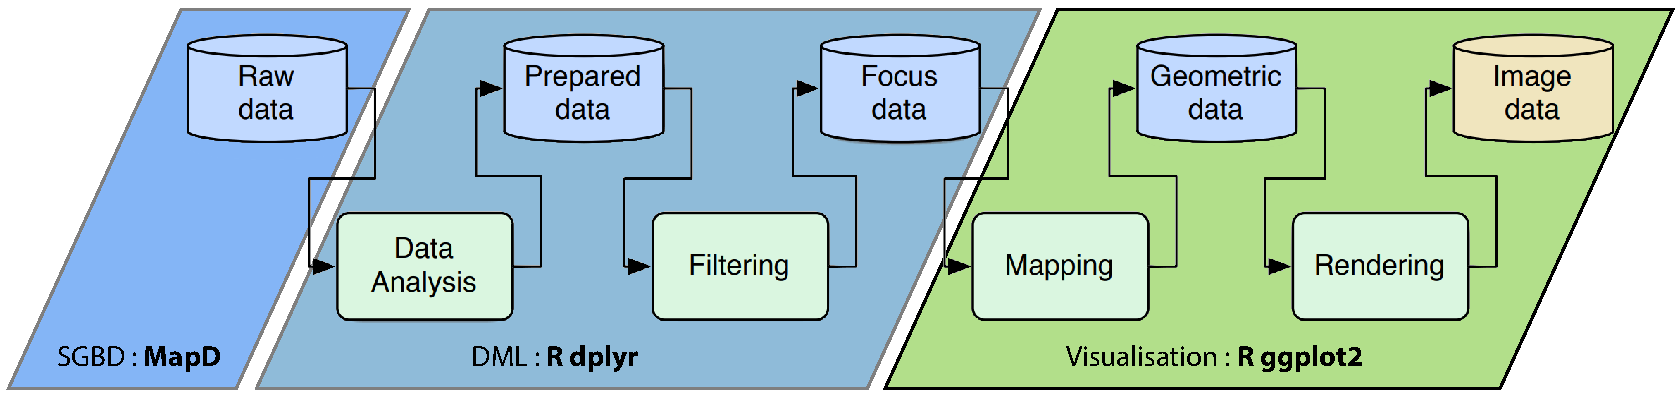
\includegraphics[width=\linewidth]{img/Visualisation_Pipeline_SimEDB.pdf}}
\hspace{5pt}
\subfloat[Une implémentation d'un exemple de pipeline de visualisation pour construire un indicateur dans SimEDB]{\label{subfig:exemple-pipeline-simedb}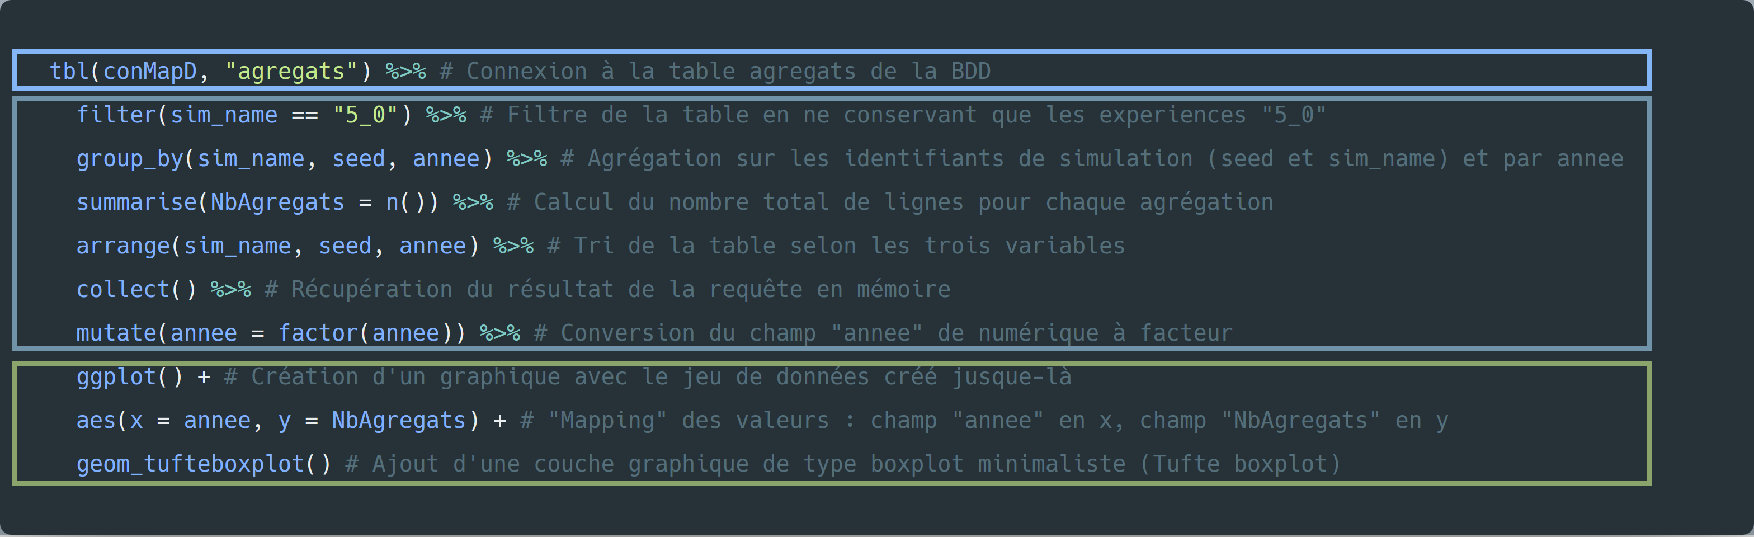
\includegraphics[width=\linewidth]{img/simedb_pipeline_R.pdf}}
\caption{\og \textit{Visualisation Pipeline}\fg{} et son implémentation dans SimEDB, en \og connectant\fg{} les codes des \cref{fig:dml-simedb,fig:exemple-ggplot2-simedb}.}
\label{fig:visualisation-pipeline-exemple}
\end{figure}

\paragraph*{Modulariser les fonctions}

Shiny, en tant qu'outil de création d'interface graphique, bénéficie aussi d'un avantage important en matière de conception d'application web : comme ce \textit{package} est basé sur un langage de programmation modulaire, on peut logiquement créer et ré-utiliser des \og briques d'interfaces\fg{} modulaires.
Par l'utilisation de modules\footnote{\href{https://shiny.rstudio.com/articles/modules.html}{https://shiny.rstudio.com/articles/modules.html}}, il est possible de définir un ensemble d'éléments graphiques adaptatifs et de ré-utiliser tel quel cet ensemble.

Dans l'interface de SimEDB, par exemple, les indicateurs graphiques sont toujours présentés de la même manière, avec l'indicateur à gauche et des outils de téléchargement et de notation de l'indicateur sur la droite.
En termes de code, les deux indicateurs comparés dans la \cref{fig:simedb-modules} sont strictement identiques : seul un paramètre varie dans l'appel aux modules, ici les filtres appliqués sur les données.
Cela permet donc d'une part de minimiser la taille du code, mais surtout, avec la généricité apportée, de faciliter de manière considérable l'ajout ou la modification d'indicateurs.

\begin{figure}[H]
\centering
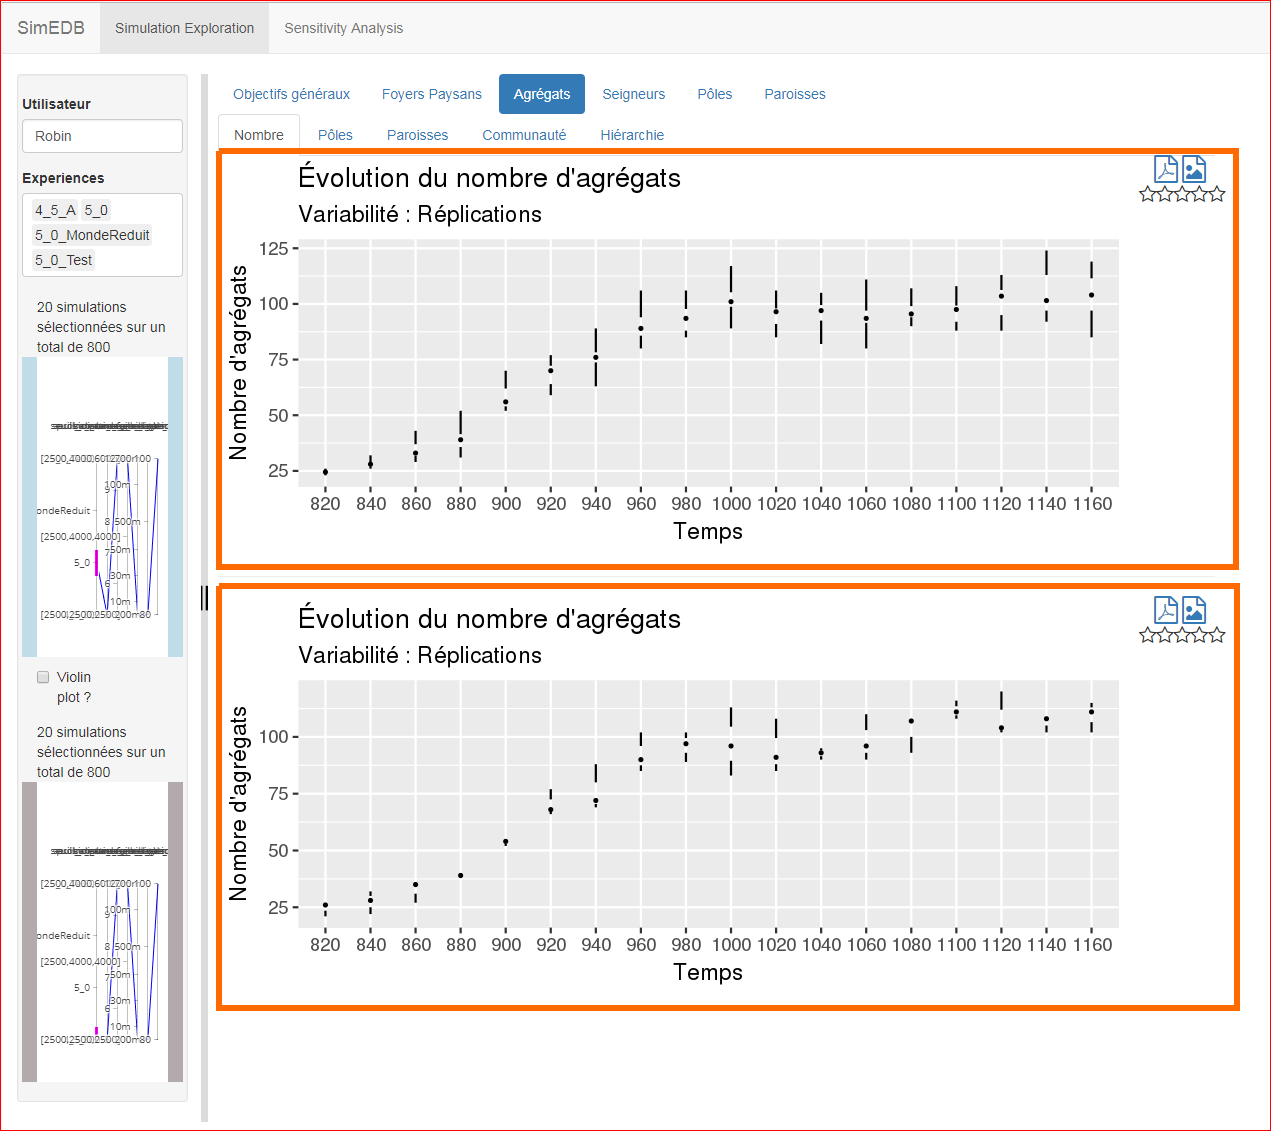
\includegraphics[width=\linewidth]{img/SimEDB_modules.png}
\caption{Une conception modulaire. Les deux éléments graphiques encadrés sont créés par un même \og module\fg{} dont les arguments varient.}
\label{fig:simedb-modules}
\end{figure}


\subsubsection{Choix de l'organisation visuelle}

Les différentes étapes de construction d'une plate-forme d'exploration (\cref{sec:explorer-sorties-simfeodal} : \cnameref{sec:explorer-sorties-simfeodal}) ont conduit à une organisation sous forme de \textit{dashboard} interactif.
La forme de ce \textit{dashboard} a évolué tout au long de l'apparition de nouveaux besoins, pour aboutir sur une organisation mono-page, pensée autour de la consultation d'indicateurs de sorties, qui devaient permettre de comparer des expériences différentes sélectionnées au moyen de graphiques en coordonnées parallèles.
Le choix d'un outil dédié à la comparaison, plus qu'à la visualisation des résultats d'un unique ensemble de simulations, entraîne nécessairement des répercussions en matière de présentation visuelle -- d'interface graphique -- des éléments permettant de mener cette comparaison.
Depuis la première plate-forme aboutie -- SimVADB (voir \cref{fig:simvadb_dashboard}, \cpageref{fig:simvadb_dashboard}) --, l'interface graphique a donc fortement évolué.

\paragraph*{Une comparaison verticale}

En premier lieu, on peut remarquer que les \og contrôleurs\fg{}, c'est-à-dire les graphiques interactifs en coordonnées parallèles ainsi que de nouveaux menus de sélections (\cref{fig:simedb-sidebar}) ne sont plus dans la partie supérieure de l'interface, mais dans la partie latérale de l'application.

Le choix prédominant à cette modification est la volonté de comparaison : dans SimVADB, on pouvait déjà comparer deux graphiques, mais ceux-ci étaient alors côte-à-côte.
Étant donné que l'axe des ordonnées est dépendant de chaque graphique -- on ne peut attribuer de limites communes à chaque graphique sans avoir à recalculer chacun des indicateurs à chaque changement de sélection de l'un ou de l'autre --, une comparaison visuelle des positions en ordonnées des courbes et marqueurs n'a pas véritablement de sens.
Au contraire, le plus souvent, l'axe des abscisses est fixe : qu'il représente le temps (nombre d'agrégats par pas de temps\ldots), une discrétisation de valeurs continues (composition en attracteurs des pôles\ldots), ou encore les différentes modalités d'une variable (détail du déplacement des foyers paysans\ldots), l'étendu et la composition des éléments en abscisse est généralement prévisible.

Avec un axe \og fixe\fg{}, il est donc opportun de mener la comparaison visuelle sur cet axe, et donc d'aligner les graphiques sur celui-ci. L'organisation des différents indicateurs est donc verticale plutôt qu'horizontale.

\begin{figure}[H]
\centering
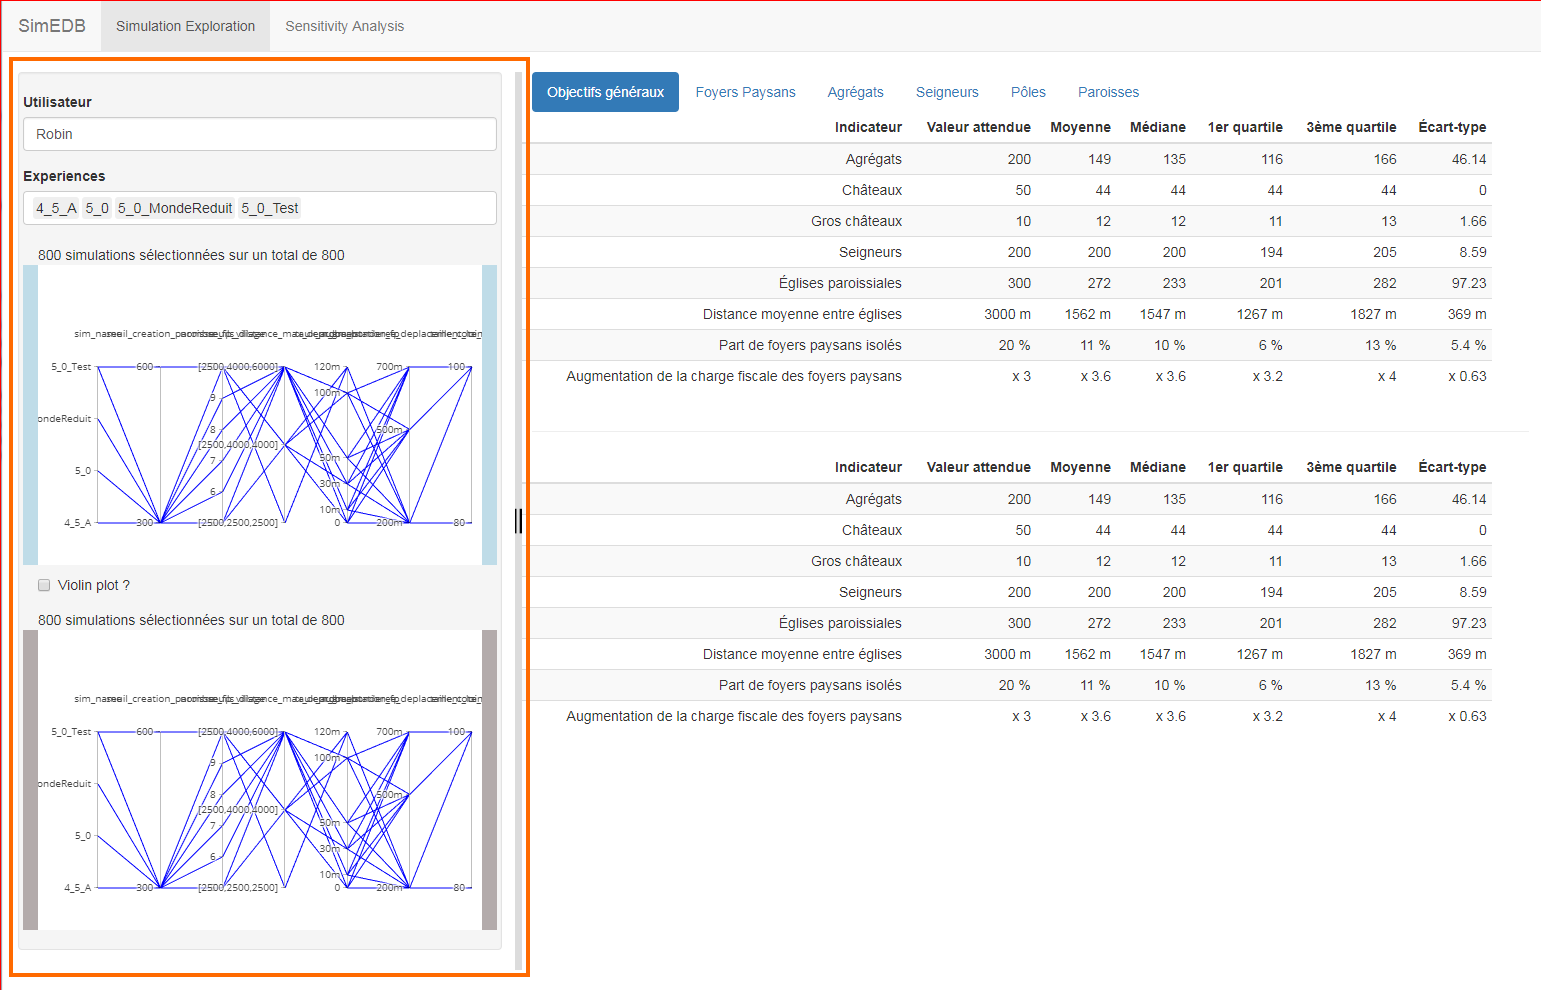
\includegraphics[width=\linewidth]{img/SimEDB_sidebar_cut.png}
\caption{La barre de contrôleurs dans l'interface de SimEDB}
\label{fig:simedb-sidebar}
\end{figure}

Afin que la sélection des simulations à explorer soit intuitive, les contrôleurs doivent donc être alignés face à cet agencement vertical des indicateurs, et dès lors, verticalisés eux aussi.

Pour bien différencier visuellement ce qui relève d'un affichage et ce qui requiert une interaction, les contrôleurs s'inscrivent dans un panneau dédié, grisé, ce qui constitue presque un standard dans les interfaces modernes d'applications interactives.

\paragraph*{Onglets et sous-onglets}

Comme dans SimVADB (\cref{subsubsec:simvadb}, \cpageref{subsubsec:simvadb}), on a choisi de conserver une navigation entre indicateurs par un systèmes d'onglets imbriqués : un premier niveau d'onglets permet d'accéder au type d'agents concernés par les indicateurs, et un second niveau permet de sélectionner spécifiquement l'indicateur choisi.
On aurait pu privilégier une vision globale, par exemple en affichant d'un coup, pour chaque type d'agents, l'ensemble des indicateurs concernés.
Sur des écrans de grande dimension, cela aurait permis d'embrasser du regard les résultats propres à chaque type d'agent bien plus rapidement, et d'accélérer d'autant l'évaluation de simulations ou leur comparaison.
La majorité des utilisateurs potentiels de SimEDB consultent toutefois l'application sur des ordinateurs portables, dotés d'écran réduits et d'une résolution faible.
L'encombrement visuel est alors atteint rapidement, et mieux vaut présenter un indicateur à la fois : la démarche visuelle sera plus longue, mais ne sera pas gênée ou faussée par des graphiques de dimension trop réduites qui peuvent induire des erreurs de lecture.

L'organisation des onglets en eux-mêmes pose aussi une question importante : vaut-il mieux organiser la consultation par type d'agent, ou plutôt, hiérarchiquement, selon la catégorie de processus examinée (\hl{à corriger une fois fixé sur le terme}, \hl{faire ref au chap3}), par exemple en respectant l'ordre de consultation des indicateurs déterminé ?

Les deux approches présentent des avantages, mais nous avons choisi de rendre l'utilisation de SimEDB plus intuitive à tous, c'est-à-dire en organisant les indicateurs par type d'agents, plutôt qu'efficace, pour les utilisateurs habitués qui auraient bénéficié d'une organisation structurée hiérarchiquement.

\subsubsection{Choix des modes d'interactions}

Avant même la conception de SimEDB, avec la plate-forme SimVADB, nous avions décidé de baser la sélection des simulations sur des graphiques en coordonnées parallèles interactifs (\cref{subsec:explo-interactive} : \cnameref{subsec:explo-interactive}).
La logique d'ensemble du filtrage de simulations restant la même, il n'était pas nécessaire de modifier ce choix pour SimEDB.

L'accumulation d'expériences, reposant sur les variations de paramètres différents, ainsi que la démultiplication des paramètres du modèle SimFeodal ayant accompagné son paramétrage, ont pourtant demandé de reconsidérer l'usage de ces graphiques interactifs.
Là où seuls quelques paramètres étaient mobilisés auparavant, les graphiques en coordonnées parallèles reposaient sur peu d'axes.
Avec l'augmentation du nombre d'axes, le graphique en coordonnées parallèle est rapidement devenu illisible faute à une surcharge graphique due au recouvrement des axes.

\paragraph*{Réduire la surcharge visuelle des graphiques en coordonnées parallèles}

La première mesure pour y remédier a été de filtrer les paramètres affichés : nul besoin d'afficher un axe correspondant à un paramètre qui n'est jamais manipulé dans les expériences.
Plutôt que de définir les paramètres \og utiles\fg{}, et donc d'avoir à les redéfinir dans l'application à chaque ajout d'expérience qui reposerait sur la variation d'un paramètre différent, nous avons fait en sorte que cette discrimination des paramètres \og actifs\fg{} soit exécutée de manière automatique :
quand SimEDB est lancé, une requête est exécutée sur la table des paramètres pour identifier ceux qui présentent plusieurs modalités et ceux qui n'en ont qu'une.
Seuls sont alors affichés les paramètres de la première catégorie, car eux-seuls présent un intérêt à être discriminés.

Ce faisant, le nombre de  paramètre affichés devient plus réduit, et permet d'afficher leurs intitulés plutôt que de faire appel à une table de correspondance comme dans SimVADB.
L'automatisation de ce traitement permet de plus de ne pas avoir à changer quoi que ce soit à la plate-forme lors d'ajouts ou de suppressions de simulations de la base de données, ce qui concoure à l'objectif d'indépendance aux données de la plate-forme d'exploration.

\paragraph*{Pré-filtrer les simulations}

Au fur et à mesure du paramétrage puis de la calibration de SimFeodal, les expériences ont tout de même continué à mobiliser de plus en plus de paramètres différents.
Pour réduire la quantité d'information représentée et améliorer en conséquence \og l'expérience utilisateur\fg{}, nous avons ajouté un filtre, moins visuel que les graphiques en coordonnées parallèle, qui permet toutefois de restreindre le nombre de simulations affichées à partir de leur dénomination.
Plutôt que de cibler des valeurs spécifiques de paramètres, l'idée est donc de soustraire des choix possibles des expériences entières.
Pour SimEDB, on a donc ajouté un pré-filtrage, sous forme de \og boîte de sélection\fg{} (\textit{select input}, \cref{fig:simedb-prefilter}), qui interroge la base de données directement pour connaître les différents intitulés de simulations et agit comme un premier filtre réduisant donc les simulations interrogées dans les graphiques en coordonnées parallèles.

\begin{figure}[H]
\centering
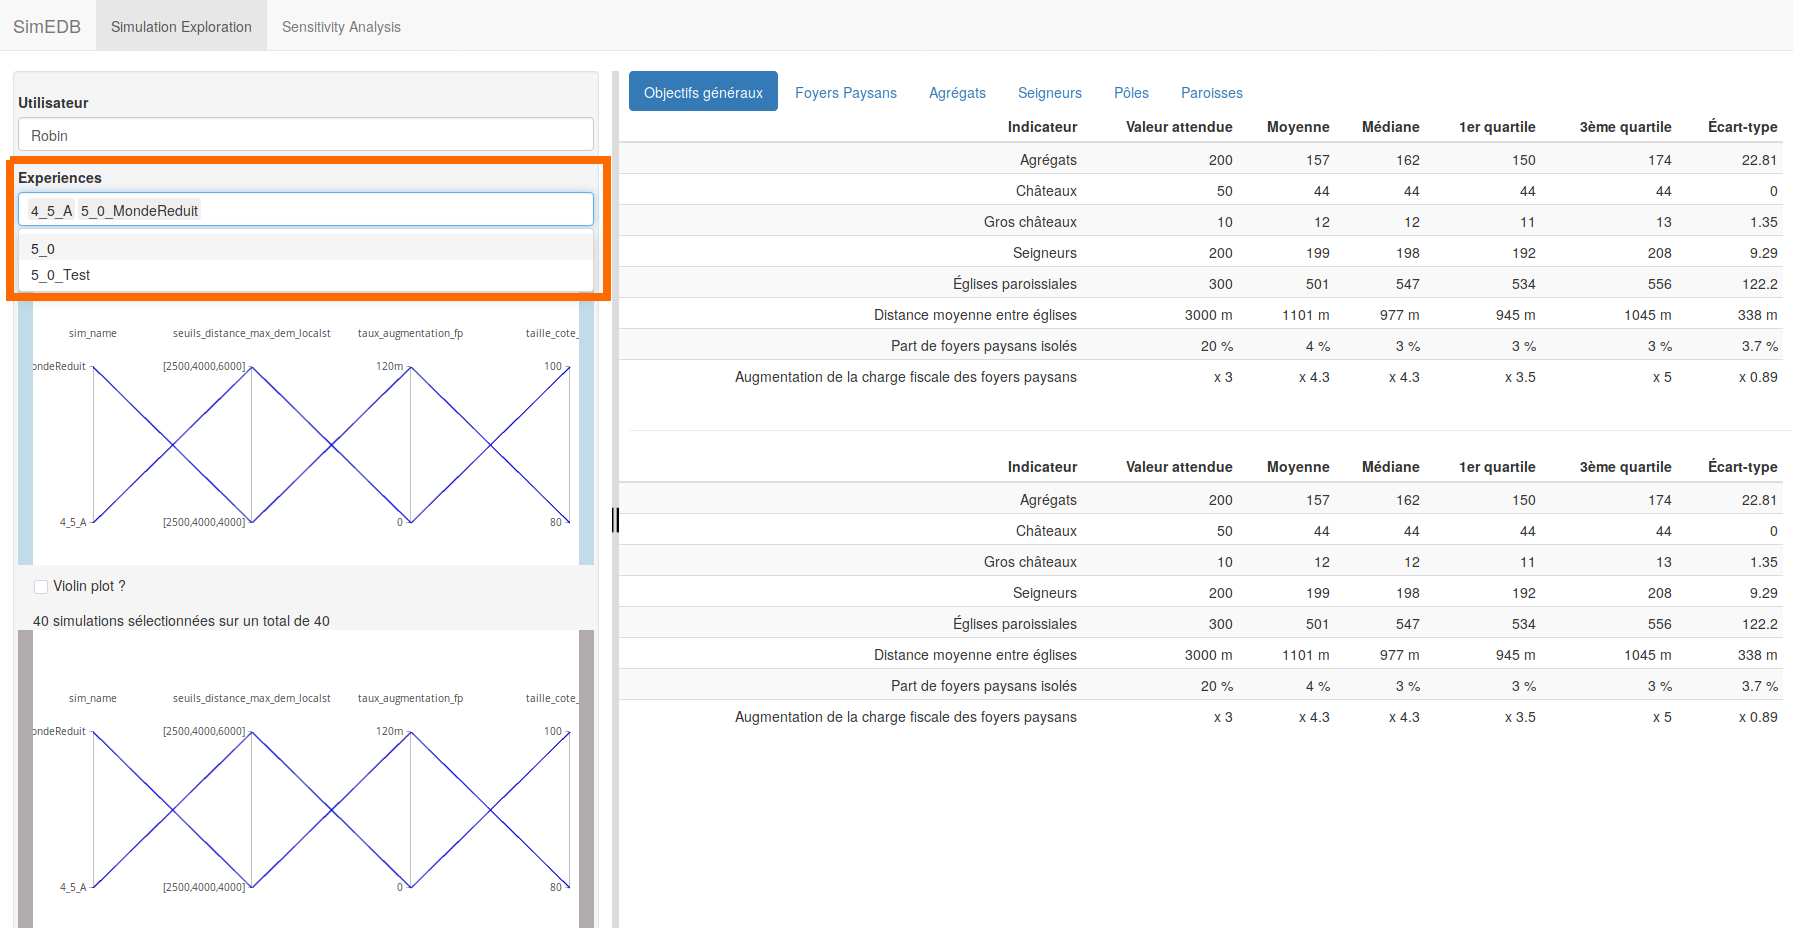
\includegraphics[width=\linewidth]{img/SimEDB_prefiltrage.png}
\caption{Le menu de sélection des expériences qui permet un pré-filtrage des expériences à partir de leur nom}
\label{fig:simedb-prefilter}
\end{figure}

\paragraph*{Optimiser l'occupation de l'espace visuel}

En dépit de ces différentes techniques visant à minimiser le nombre d'axes affichées dans les graphiques en coordonnées parallèles, la place prise par ces graphiques reste importante, en particulier quand on décide de ne pas diminuer la taille des éléments de légende afin de conserver leur lisibilité.
Quand l'application est consultée sur un écran de taille faible, l'appréhension de l'ensemble des informations présentes dans l'interface pose ainsi un véritable problème.

En réfléchissant aux séquences d'usages, par les utilisateurs, de SimEDB, on a pu comprendre que le mode d'utilisation le plus classique était de bien considérer le filtrage à effectuer sur les graphiques en coordonnées parallèles, en y consacrant un temps certain, avant de comparer longuement les différents indicateurs de la sélection.
Il n'est donc que rarement fait usage de multiples filtres successifs sur un seul indicateur, dans une approche plus exploratoire donc, mais plutôt d'évaluations complètes de simulations choisies.

Il n'est alors plus indispensable de consacrer une part importante de l'espace aux zones interactives (le panneau de contrôle), ou du moins, pas pendant l'ensemble de la période d'évaluation des simulations.

Un outil de redimensionnement a alors été ajouté à SimEDB, permettant, par glisser-déposer, de modifier la largeur occupée par le panneau de contrôle en l'adaptant à chaque moment au besoin de visualisation.
La \cref{fig:resizing} montre ainsi une succession d'états : en début d'exploration, l'utilisateur va augmenter la taille du panneau de contrôle pour augmenter la lisibilité des graphiques en coordonnées parallèles et effectuer une sélection plus simplement.
Une fois la sélection effectuée, il pourra alors re-diminuer la largeur du panneau afin d'augmenter la zone disponible, et donc la taille, pour les indicateurs de sorties de simulation. 

\begin{figure}[H]
\hspace*{\fill}%
\begin{minipage}[t]{.49\linewidth}
\centering
\vspace{0pt}
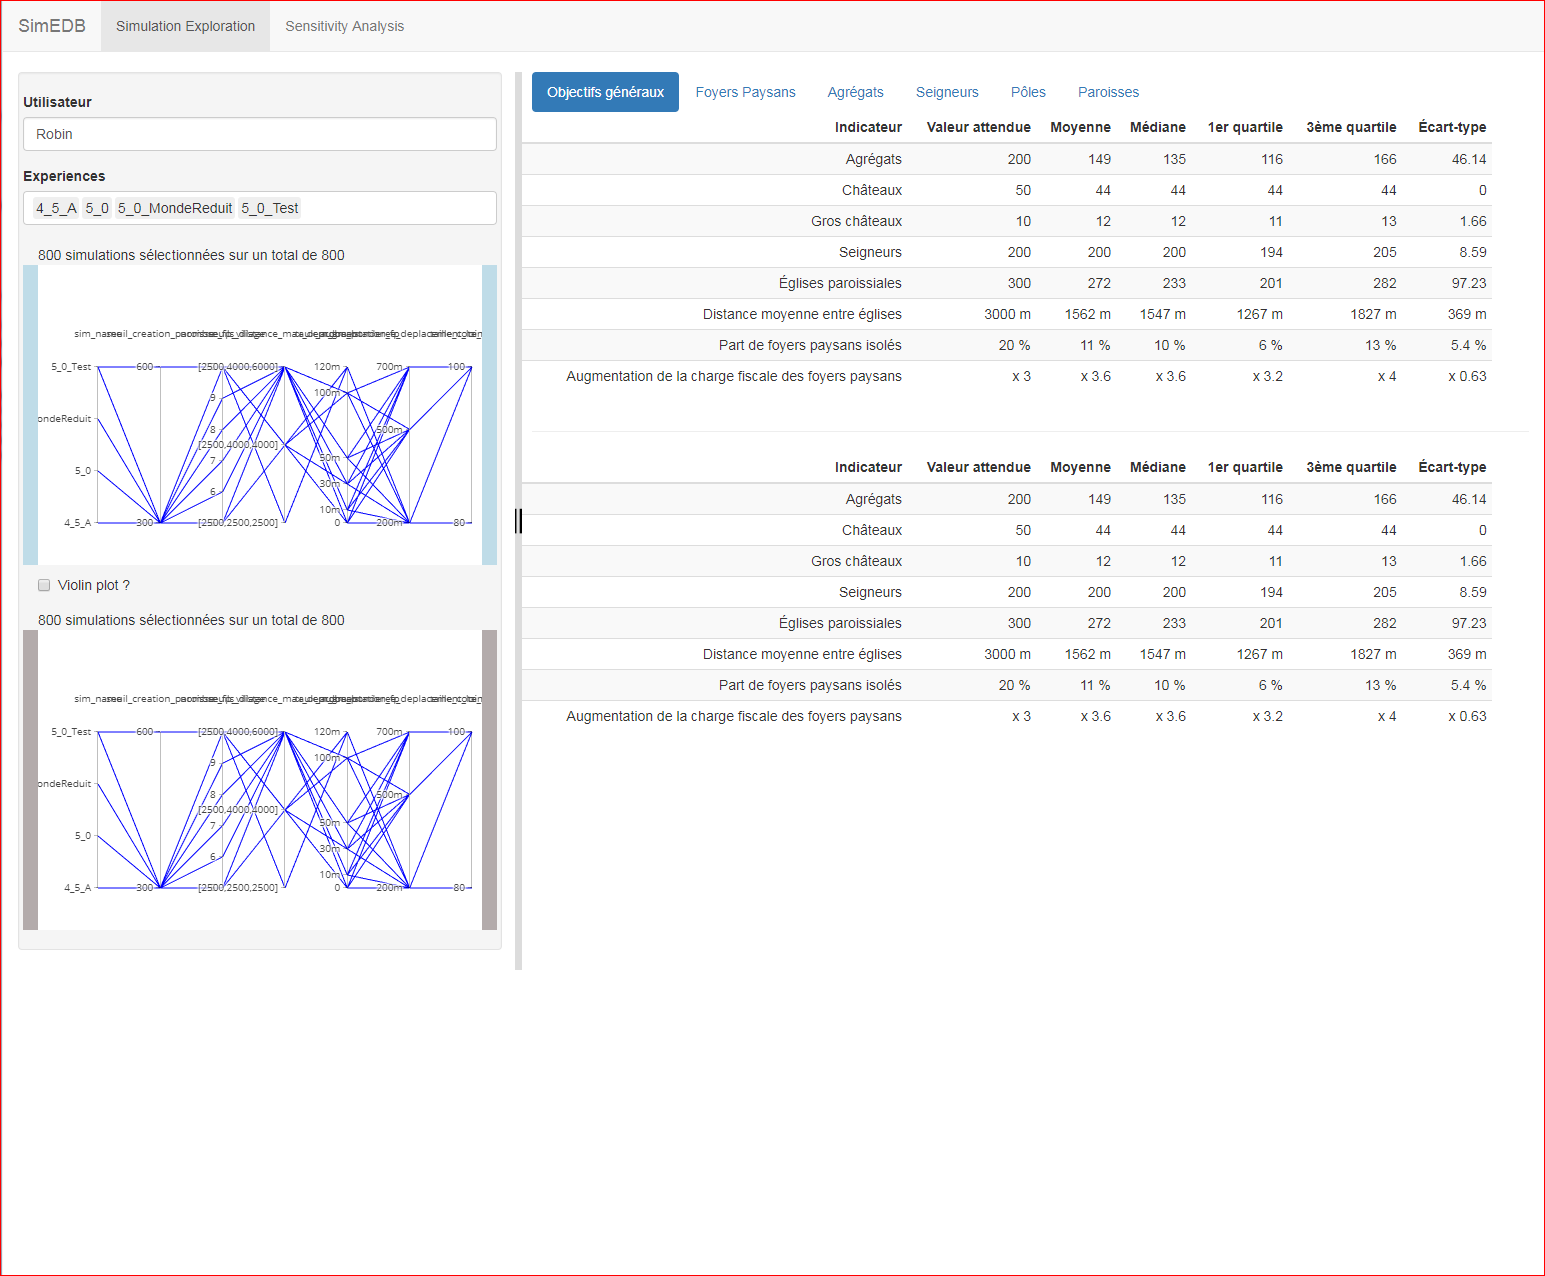
\includegraphics[width=\linewidth]{img/SimEDB_base.png}
\end{minipage} \hfill
\begin{minipage}[t]{.49\linewidth}
\centering
\vspace{0pt}
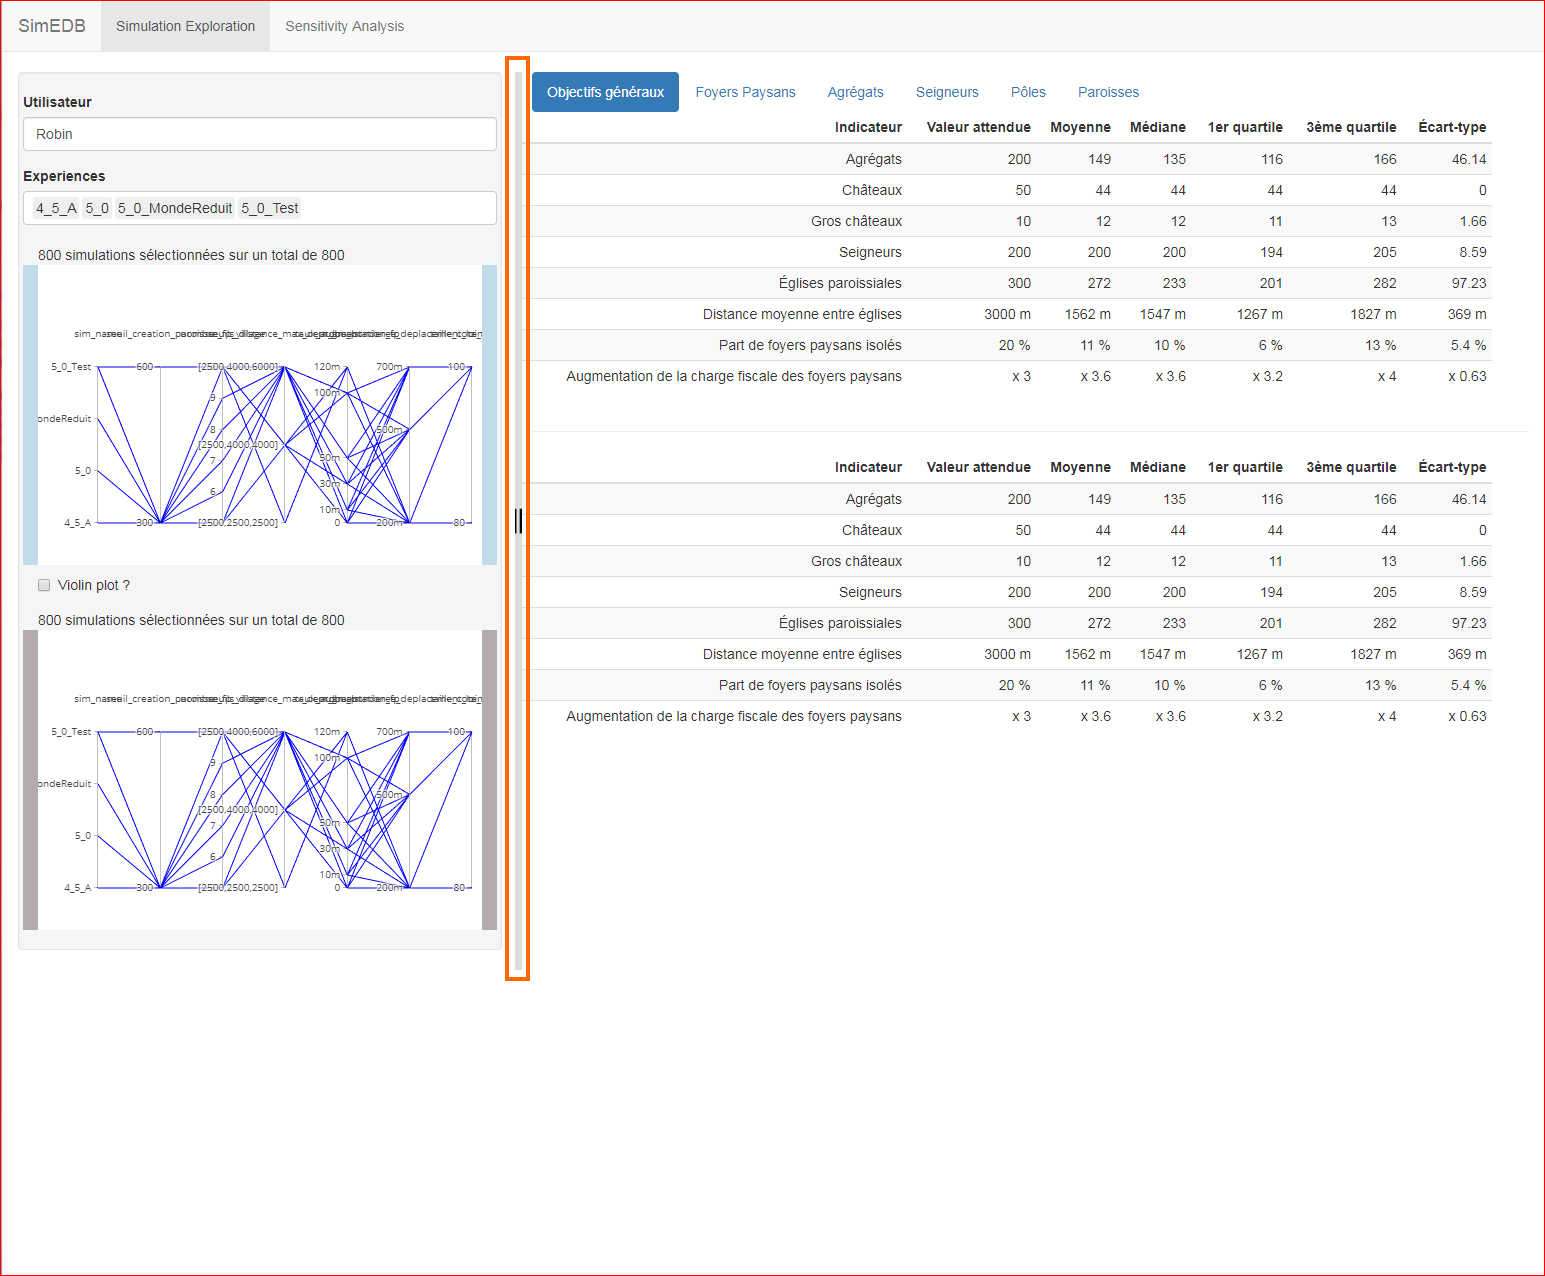
\includegraphics[width=\linewidth]{img/SimEDB_resize.png}
\end{minipage} \hfill
\begin{minipage}[b]{.49\linewidth}
\centering
\vspace{0pt}
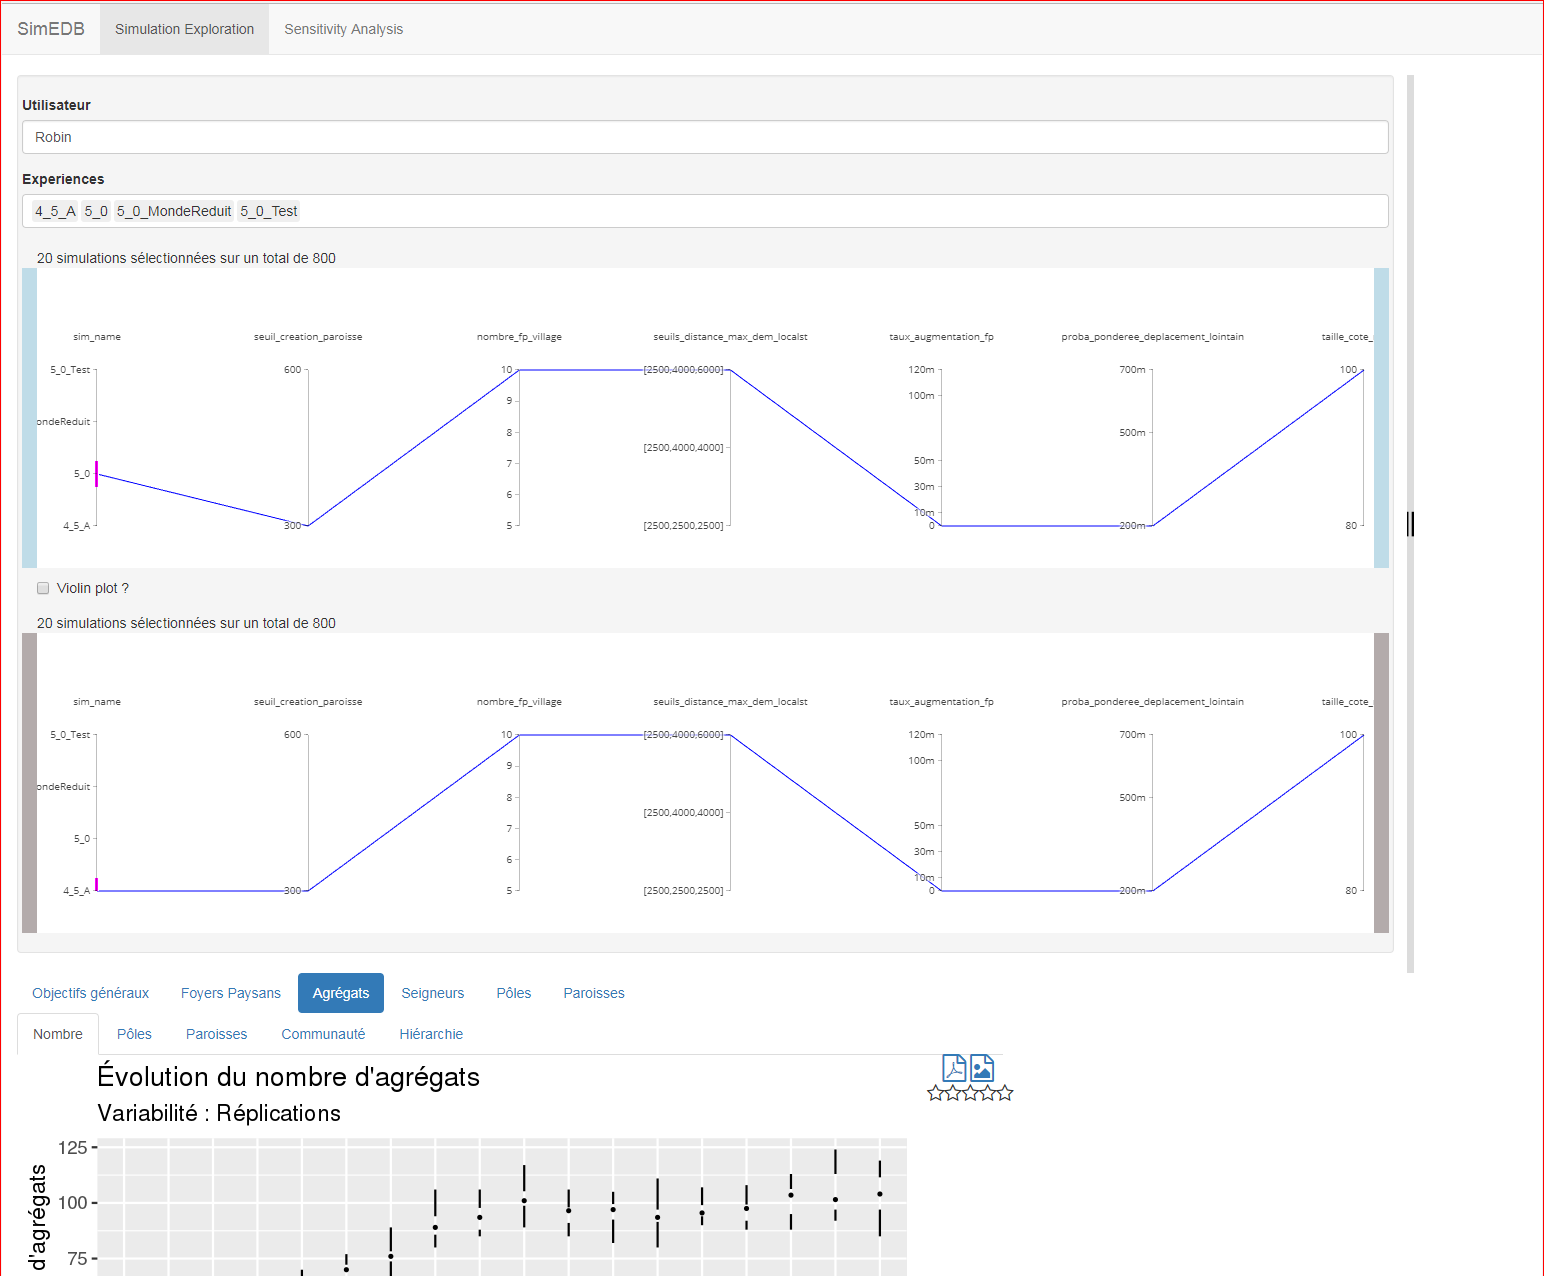
\includegraphics[width=\linewidth]{img/SimEDB_selection.png}
\end{minipage} \hfill
\begin{minipage}[b]{.49\linewidth}
\centering
\vspace{0pt}
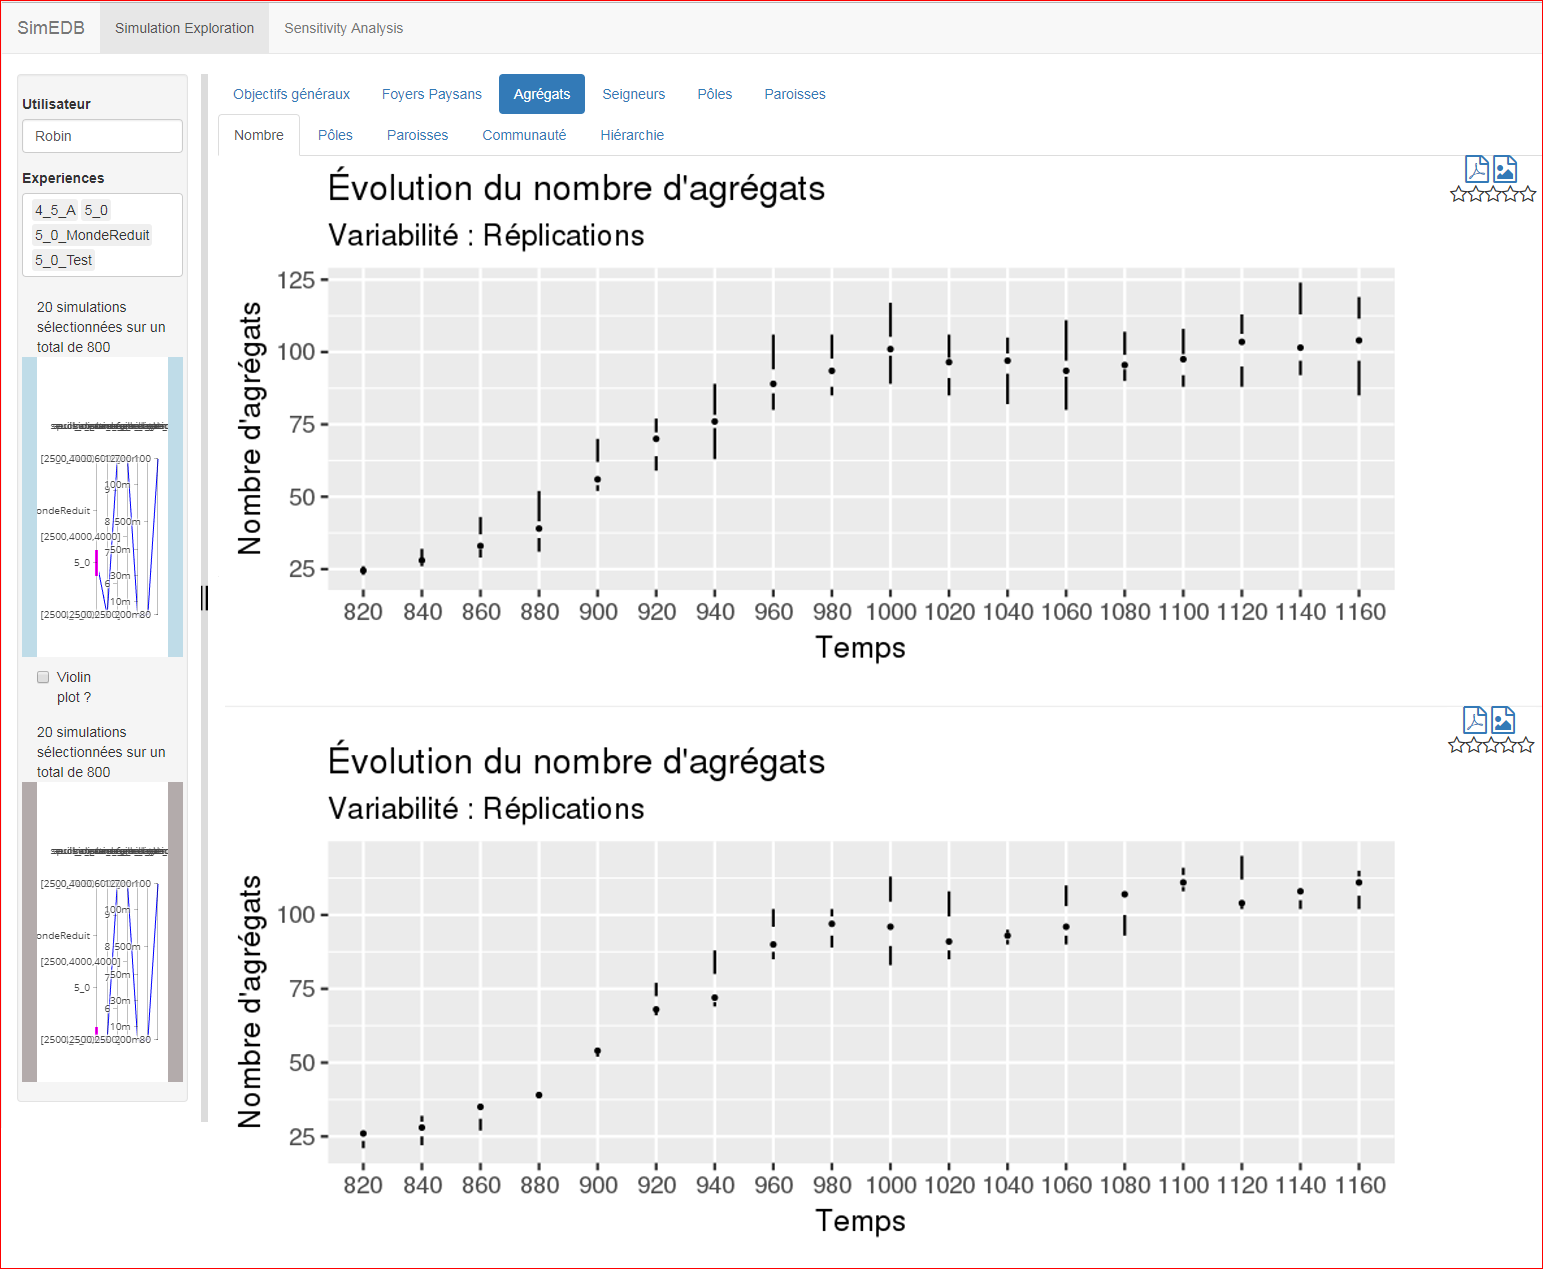
\includegraphics[width=\linewidth]{img/SimEDB_indicateur_grand_magnified.png}
\end{minipage}
\caption{Utilisation interactive de SimEDB et redimensionnement du panneau de contrôle.}
\label{fig:resizing}
\end{figure}

\paragraph*{Répondre aux demandes des utilisateurs : ajout d'un mécanisme d'export des indicateurs}

L'intérêt d'une interface modulaire et factorisée se révèle véritablement quand les utilisateurs d'un outil demandent des fonctionnalités supplémentaires, non prévues lors de la conception de l'outil.
Dans le cas de SimFeodal, une telle requête est rapidement apparue : les thématiciens, mais aussi les modélisateurs, pour conserver une trace d'une session d'exploration des indicateurs, souhaitaient pouvoir exporter les graphiques correspondant aux indicateurs.
Si au départ, une simple capture d'écran pouvait suffire, ce besoin a été complété par une volonté d'inclure des indicateurs de simulations dans des articles et autres communications, requérant donc des retouches des graphiques.
Pour ce faire, on a choisi d'ajouter des fonctionnalités de téléchargement des graphiques, selon deux formats -- image et vectoriel -- afin de satisfaire à ces deux usages.
Avec le développement modulaire adopté, il a suffit d'ajouter ces fonctions d'export en un unique lieu dans le code-source de SimEDB, et l'ajout de ces nouvelles fonctionnalités a alors été disponible automatiquement pour chacun des indicateurs graphiques.

\medskip
\hl{Ajouter un paragraphe, plus tard, sur l'inscription des modalités de filtrage (quelles sont les filtres appliqués ?) dans les graphiques, si j'arrive à trouver le temps de l'ajouter un jour...}

\paragraph*{Noter les simulations}

Un dernier point d'interaction avec l'application a été prévu, sans pouvoir toutefois être mobilisé jusque là : il s'agissait d'aller vers une semi-automatisation de l'évaluation des simulations, par l'intermédiaire d'un outil graphique permettant de \og noter\fg{} les simulations sélectionnées.
Pour ce faire, et parce que, on l'a vu, l'évaluation d'un ensemble de simulations ne peut se faire de manière unique, on a choisi de donner la possibilité aux utilisateurs experts de noter chacun des indicateurs de sortie, pour chacun des ensembles de simulations qu'ils exploreraient.
L'évaluation se fait au moyen d'un outil simple, composé de 5 \og étoiles\fg{}, et est enregistré à chaque nouvelle note.

Une piste d'utilisation serait de mobiliser les données ainsi créées, composées d'une note donnée à un indicateur pour un ensemble d'identifiants uniques de simulations, afin de réaliser des analyses quantitatives des notes attribuées : est-ce que certaines simulations sont systématiquement bien notées avec chacun des indicateurs affichés ? Certains indicateurs ne sont-ils jamais observés ou ne donnent-ils jamais lieu à évaluation ?

Cette fonctionnalité, bien qu'implémentée, n'est pas encore utilisée, mais devrait à terme permettre d'aller vers une meilleure connaissance des résultats de simulation, tout autant que vers une mesure de l'efficacité des indicateurs de sortie choisis pour évaluer un ensemble de simulations.

\subsubsection{Présentation générale}

\begin{itemize}
\item \hl{Quelques captures d'écran successives avec focus à chaque fois sur l'interaction en cours, ou alors,}
\item \hl{renvoyer à un manuel utilisateur en annexe, ou alors,}
\item \hl{ajouter un tuto interactif à l'application et en mettre le lien + descriptif ici}
\end{itemize}
